\PassOptionsToPackage{table}{xcolor}
\documentclass{template}
\usepackage[fontset=fandol,UTF8]{ctex}

\usepackage{mathtools}
\usepackage{multirow}
\usepackage{bm}
\usepackage{placeins}
\usepackage{etoolbox}

\usepackage{amsmath,amsfonts,bm}

\newcommand{\figleft}{{\em (Left)}}
\newcommand{\figcenter}{{\em (Center)}}
\newcommand{\figright}{{\em (Right)}}
\newcommand{\figtop}{{\em (Top)}}
\newcommand{\figbottom}{{\em (Bottom)}}
\newcommand{\captiona}{{\em (a)}}
\newcommand{\captionb}{{\em (b)}}
\newcommand{\captionc}{{\em (c)}}
\newcommand{\captiond}{{\em (d)}}

\newcommand{\newterm}[1]{{\bf #1}}


\def\figref#1{figure~\ref{#1}}
\def\Figref#1{Figure~\ref{#1}}
\def\twofigref#1#2{figures \ref{#1} and \ref{#2}}
\def\quadfigref#1#2#3#4{figures \ref{#1}, \ref{#2}, \ref{#3} and \ref{#4}}
\def\secref#1{section~\ref{#1}}
\def\Secref#1{Section~\ref{#1}}
\def\twosecrefs#1#2{sections \ref{#1} and \ref{#2}}
\def\secrefs#1#2#3{sections \ref{#1}, \ref{#2} and \ref{#3}}
\def\eqref#1{equation~\ref{#1}}
\def\Eqref#1{Equation~\ref{#1}}
\def\plaineqref#1{\ref{#1}}
\def\chapref#1{chapter~\ref{#1}}
\def\Chapref#1{Chapter~\ref{#1}}
\def\rangechapref#1#2{chapters\ref{#1}--\ref{#2}}
\def\algref#1{algorithm~\ref{#1}}
\def\Algref#1{Algorithm~\ref{#1}}
\def\twoalgref#1#2{algorithms \ref{#1} and \ref{#2}}
\def\Twoalgref#1#2{Algorithms \ref{#1} and \ref{#2}}
\def\partref#1{part~\ref{#1}}
\def\Partref#1{Part~\ref{#1}}
\def\twopartref#1#2{parts \ref{#1} and \ref{#2}}

\def\ceil#1{\lceil #1 \rceil}
\def\floor#1{\lfloor #1 \rfloor}
\def\1{\bm{1}}
\newcommand{\train}{\mathcal{D}}
\newcommand{\valid}{\mathcal{D_{\mathrm{valid}}}}
\newcommand{\test}{\mathcal{D_{\mathrm{test}}}}

\def\eps{{\epsilon}}


\def\reta{{\textnormal{$\eta$}}}
\def\ra{{\textnormal{a}}}
\def\rb{{\textnormal{b}}}
\def\rc{{\textnormal{c}}}
\def\rd{{\textnormal{d}}}
\def\re{{\textnormal{e}}}
\def\rf{{\textnormal{f}}}
\def\rg{{\textnormal{g}}}
\def\rh{{\textnormal{h}}}
\def\ri{{\textnormal{i}}}
\def\rj{{\textnormal{j}}}
\def\rk{{\textnormal{k}}}
\def\rl{{\textnormal{l}}}
\def\rn{{\textnormal{n}}}
\def\ro{{\textnormal{o}}}
\def\rp{{\textnormal{p}}}
\def\rq{{\textnormal{q}}}
\def\rr{{\textnormal{r}}}
\def\rs{{\textnormal{s}}}
\def\rt{{\textnormal{t}}}
\def\ru{{\textnormal{u}}}
\def\rv{{\textnormal{v}}}
\def\rw{{\textnormal{w}}}
\def\rx{{\textnormal{x}}}
\def\ry{{\textnormal{y}}}
\def\rz{{\textnormal{z}}}

\def\rvepsilon{{\mathbf{\epsilon}}}
\def\rvtheta{{\mathbf{\theta}}}
\def\rva{{\mathbf{a}}}
\def\rvb{{\mathbf{b}}}
\def\rvc{{\mathbf{c}}}
\def\rvd{{\mathbf{d}}}
\def\rve{{\mathbf{e}}}
\def\rvf{{\mathbf{f}}}
\def\rvg{{\mathbf{g}}}
\def\rvh{{\mathbf{h}}}
\def\rvu{{\mathbf{i}}}
\def\rvj{{\mathbf{j}}}
\def\rvk{{\mathbf{k}}}
\def\rvl{{\mathbf{l}}}
\def\rvm{{\mathbf{m}}}
\def\rvn{{\mathbf{n}}}
\def\rvo{{\mathbf{o}}}
\def\rvp{{\mathbf{p}}}
\def\rvq{{\mathbf{q}}}
\def\rvr{{\mathbf{r}}}
\def\rvs{{\mathbf{s}}}
\def\rvt{{\mathbf{t}}}
\def\rvu{{\mathbf{u}}}
\def\rvv{{\mathbf{v}}}
\def\rvw{{\mathbf{w}}}
\def\rvx{{\mathbf{x}}}
\def\rvy{{\mathbf{y}}}
\def\rvz{{\mathbf{z}}}

\def\erva{{\textnormal{a}}}
\def\ervb{{\textnormal{b}}}
\def\ervc{{\textnormal{c}}}
\def\ervd{{\textnormal{d}}}
\def\erve{{\textnormal{e}}}
\def\ervf{{\textnormal{f}}}
\def\ervg{{\textnormal{g}}}
\def\ervh{{\textnormal{h}}}
\def\ervi{{\textnormal{i}}}
\def\ervj{{\textnormal{j}}}
\def\ervk{{\textnormal{k}}}
\def\ervl{{\textnormal{l}}}
\def\ervm{{\textnormal{m}}}
\def\ervn{{\textnormal{n}}}
\def\ervo{{\textnormal{o}}}
\def\ervp{{\textnormal{p}}}
\def\ervq{{\textnormal{q}}}
\def\ervr{{\textnormal{r}}}
\def\ervs{{\textnormal{s}}}
\def\ervt{{\textnormal{t}}}
\def\ervu{{\textnormal{u}}}
\def\ervv{{\textnormal{v}}}
\def\ervw{{\textnormal{w}}}
\def\ervx{{\textnormal{x}}}
\def\ervy{{\textnormal{y}}}
\def\ervz{{\textnormal{z}}}

\def\rmA{{\mathbf{A}}}
\def\rmB{{\mathbf{B}}}
\def\rmC{{\mathbf{C}}}
\def\rmD{{\mathbf{D}}}
\def\rmE{{\mathbf{E}}}
\def\rmF{{\mathbf{F}}}
\def\rmG{{\mathbf{G}}}
\def\rmH{{\mathbf{H}}}
\def\rmI{{\mathbf{I}}}
\def\rmJ{{\mathbf{J}}}
\def\rmK{{\mathbf{K}}}
\def\rmL{{\mathbf{L}}}
\def\rmM{{\mathbf{M}}}
\def\rmN{{\mathbf{N}}}
\def\rmO{{\mathbf{O}}}
\def\rmP{{\mathbf{P}}}
\def\rmQ{{\mathbf{Q}}}
\def\rmR{{\mathbf{R}}}
\def\rmS{{\mathbf{S}}}
\def\rmT{{\mathbf{T}}}
\def\rmU{{\mathbf{U}}}
\def\rmV{{\mathbf{V}}}
\def\rmW{{\mathbf{W}}}
\def\rmX{{\mathbf{X}}}
\def\rmY{{\mathbf{Y}}}
\def\rmZ{{\mathbf{Z}}}

\def\ermA{{\textnormal{A}}}
\def\ermB{{\textnormal{B}}}
\def\ermC{{\textnormal{C}}}
\def\ermD{{\textnormal{D}}}
\def\ermE{{\textnormal{E}}}
\def\ermF{{\textnormal{F}}}
\def\ermG{{\textnormal{G}}}
\def\ermH{{\textnormal{H}}}
\def\ermI{{\textnormal{I}}}
\def\ermJ{{\textnormal{J}}}
\def\ermK{{\textnormal{K}}}
\def\ermL{{\textnormal{L}}}
\def\ermM{{\textnormal{M}}}
\def\ermN{{\textnormal{N}}}
\def\ermO{{\textnormal{O}}}
\def\ermP{{\textnormal{P}}}
\def\ermQ{{\textnormal{Q}}}
\def\ermR{{\textnormal{R}}}
\def\ermS{{\textnormal{S}}}
\def\ermT{{\textnormal{T}}}
\def\ermU{{\textnormal{U}}}
\def\ermV{{\textnormal{V}}}
\def\ermW{{\textnormal{W}}}
\def\ermX{{\textnormal{X}}}
\def\ermY{{\textnormal{Y}}}
\def\ermZ{{\textnormal{Z}}}

\def\vzero{{\bm{0}}}
\def\vone{{\bm{1}}}
\def\vmu{{\bm{\mu}}}
\def\vtheta{{\bm{\theta}}}
\def\va{{\bm{a}}}
\def\vb{{\bm{b}}}
\def\vc{{\bm{c}}}
\def\vd{{\bm{d}}}
\def\ve{{\bm{e}}}
\def\vf{{\bm{f}}}
\def\vg{{\bm{g}}}
\def\vh{{\bm{h}}}
\def\vi{{\bm{i}}}
\def\vj{{\bm{j}}}
\def\vk{{\bm{k}}}
\def\vl{{\bm{l}}}
\def\vm{{\bm{m}}}
\def\vn{{\bm{n}}}
\def\vo{{\bm{o}}}
\def\vp{{\bm{p}}}
\def\vq{{\bm{q}}}
\def\vr{{\bm{r}}}
\def\vs{{\bm{s}}}
\def\vt{{\bm{t}}}
\def\vu{{\bm{u}}}
\def\vv{{\bm{v}}}
\def\vw{{\bm{w}}}
\def\vx{{\bm{x}}}
\def\vy{{\bm{y}}}
\def\vz{{\bm{z}}}

\def\evalpha{{\alpha}}
\def\evbeta{{\beta}}
\def\evepsilon{{\epsilon}}
\def\evlambda{{\lambda}}
\def\evomega{{\omega}}
\def\evmu{{\mu}}
\def\evpsi{{\psi}}
\def\evsigma{{\sigma}}
\def\evtheta{{\theta}}
\def\eva{{a}}
\def\evb{{b}}
\def\evc{{c}}
\def\evd{{d}}
\def\eve{{e}}
\def\evf{{f}}
\def\evg{{g}}
\def\evh{{h}}
\def\evi{{i}}
\def\evj{{j}}
\def\evk{{k}}
\def\evl{{l}}
\def\evm{{m}}
\def\evn{{n}}
\def\evo{{o}}
\def\evp{{p}}
\def\evq{{q}}
\def\evr{{r}}
\def\evs{{s}}
\def\evt{{t}}
\def\evu{{u}}
\def\evv{{v}}
\def\evw{{w}}
\def\evx{{x}}
\def\evy{{y}}
\def\evz{{z}}

\def\mA{{\bm{A}}}
\def\mB{{\bm{B}}}
\def\mC{{\bm{C}}}
\def\mD{{\bm{D}}}
\def\mE{{\bm{E}}}
\def\mF{{\bm{F}}}
\def\mG{{\bm{G}}}
\def\mH{{\bm{H}}}
\def\mI{{\bm{I}}}
\def\mJ{{\bm{J}}}
\def\mK{{\bm{K}}}
\def\mL{{\bm{L}}}
\def\mM{{\bm{M}}}
\def\mN{{\bm{N}}}
\def\mO{{\bm{O}}}
\def\mP{{\bm{P}}}
\def\mQ{{\bm{Q}}}
\def\mR{{\bm{R}}}
\def\mS{{\bm{S}}}
\def\mT{{\bm{T}}}
\def\mU{{\bm{U}}}
\def\mV{{\bm{V}}}
\def\mW{{\bm{W}}}
\def\mX{{\bm{X}}}
\def\mY{{\bm{Y}}}
\def\mZ{{\bm{Z}}}
\def\mBeta{{\bm{\beta}}}
\def\mPhi{{\bm{\Phi}}}
\def\mLambda{{\bm{\Lambda}}}
\def\mSigma{{\bm{\Sigma}}}

\DeclareMathAlphabet{\mathsfit}{\encodingdefault}{\sfdefault}{m}{sl}

\newcommand{\tens}[1]{\bm{\mathsfit{#1}}}
\def\tA{{\tens{A}}}
\def\tB{{\tens{B}}}
\def\tC{{\tens{C}}}
\def\tD{{\tens{D}}}
\def\tE{{\tens{E}}}
\def\tF{{\tens{F}}}
\def\tG{{\tens{G}}}
\def\tH{{\tens{H}}}
\def\tI{{\tens{I}}}
\def\tJ{{\tens{J}}}
\def\tK{{\tens{K}}}
\def\tL{{\tens{L}}}
\def\tM{{\tens{M}}}
\def\tN{{\tens{N}}}
\def\tO{{\tens{O}}}
\def\tP{{\tens{P}}}
\def\tQ{{\tens{Q}}}
\def\tR{{\tens{R}}}
\def\tS{{\tens{S}}}
\def\tT{{\tens{T}}}
\def\tU{{\tens{U}}}
\def\tV{{\tens{V}}}
\def\tW{{\tens{W}}}
\def\tX{{\tens{X}}}
\def\tY{{\tens{Y}}}
\def\tZ{{\tens{Z}}}


\def\gA{{\mathcal{A}}}
\def\gB{{\mathcal{B}}}
\def\gC{{\mathcal{C}}}
\def\gD{{\mathcal{D}}}
\def\gE{{\mathcal{E}}}
\def\gF{{\mathcal{F}}}
\def\gG{{\mathcal{G}}}
\def\gH{{\mathcal{H}}}
\def\gI{{\mathcal{I}}}
\def\gJ{{\mathcal{J}}}
\def\gK{{\mathcal{K}}}
\def\gL{{\mathcal{L}}}
\def\gM{{\mathcal{M}}}
\def\gN{{\mathcal{N}}}
\def\gO{{\mathcal{O}}}
\def\gP{{\mathcal{P}}}
\def\gQ{{\mathcal{Q}}}
\def\gR{{\mathcal{R}}}
\def\gS{{\mathcal{S}}}
\def\gT{{\mathcal{T}}}
\def\gU{{\mathcal{U}}}
\def\gV{{\mathcal{V}}}
\def\gW{{\mathcal{W}}}
\def\gX{{\mathcal{X}}}
\def\gY{{\mathcal{Y}}}
\def\gZ{{\mathcal{Z}}}

\def\sA{{\mathbb{A}}}
\def\sB{{\mathbb{B}}}
\def\sC{{\mathbb{C}}}
\def\sD{{\mathbb{D}}}
\def\sF{{\mathbb{F}}}
\def\sG{{\mathbb{G}}}
\def\sH{{\mathbb{H}}}
\def\sI{{\mathbb{I}}}
\def\sJ{{\mathbb{J}}}
\def\sK{{\mathbb{K}}}
\def\sL{{\mathbb{L}}}
\def\sM{{\mathbb{M}}}
\def\sN{{\mathbb{N}}}
\def\sO{{\mathbb{O}}}
\def\sP{{\mathbb{P}}}
\def\sQ{{\mathbb{Q}}}
\def\sR{{\mathbb{R}}}
\def\sS{{\mathbb{S}}}
\def\sT{{\mathbb{T}}}
\def\sU{{\mathbb{U}}}
\def\sV{{\mathbb{V}}}
\def\sW{{\mathbb{W}}}
\def\sX{{\mathbb{X}}}
\def\sY{{\mathbb{Y}}}
\def\sZ{{\mathbb{Z}}}

\def\emLambda{{\Lambda}}
\def\emA{{A}}
\def\emB{{B}}
\def\emC{{C}}
\def\emD{{D}}
\def\emE{{E}}
\def\emF{{F}}
\def\emG{{G}}
\def\emH{{H}}
\def\emI{{I}}
\def\emJ{{J}}
\def\emK{{K}}
\def\emL{{L}}
\def\emM{{M}}
\def\emN{{N}}
\def\emO{{O}}
\def\emP{{P}}
\def\emQ{{Q}}
\def\emR{{R}}
\def\emS{{S}}
\def\emT{{T}}
\def\emU{{U}}
\def\emV{{V}}
\def\emW{{W}}
\def\emX{{X}}
\def\emY{{Y}}
\def\emZ{{Z}}
\def\emSigma{{\Sigma}}

\newcommand{\etens}[1]{\mathsfit{#1}}
\def\etLambda{{\etens{\Lambda}}}
\def\etA{{\etens{A}}}
\def\etB{{\etens{B}}}
\def\etC{{\etens{C}}}
\def\etD{{\etens{D}}}
\def\etE{{\etens{E}}}
\def\etF{{\etens{F}}}
\def\etG{{\etens{G}}}
\def\etH{{\etens{H}}}
\def\etI{{\etens{I}}}
\def\etJ{{\etens{J}}}
\def\etK{{\etens{K}}}
\def\etL{{\etens{L}}}
\def\etM{{\etens{M}}}
\def\etN{{\etens{N}}}
\def\etO{{\etens{O}}}
\def\etP{{\etens{P}}}
\def\etQ{{\etens{Q}}}
\def\etR{{\etens{R}}}
\def\etS{{\etens{S}}}
\def\etT{{\etens{T}}}
\def\etU{{\etens{U}}}
\def\etV{{\etens{V}}}
\def\etW{{\etens{W}}}
\def\etX{{\etens{X}}}
\def\etY{{\etens{Y}}}
\def\etZ{{\etens{Z}}}

\newcommand{\pdata}{p_{\rm{data}}}
\newcommand{\ptrain}{\hat{p}_{\rm{data}}}
\newcommand{\Ptrain}{\hat{P}_{\rm{data}}}
\newcommand{\pmodel}{p_{\rm{model}}}
\newcommand{\Pmodel}{P_{\rm{model}}}
\newcommand{\ptildemodel}{\tilde{p}_{\rm{model}}}
\newcommand{\pencode}{p_{\rm{encoder}}}
\newcommand{\pdecode}{p_{\rm{decoder}}}
\newcommand{\precons}{p_{\rm{reconstruct}}}

\newcommand{\laplace}{\mathrm{Laplace}} 

\newcommand{\E}{\mathbb{E}}
\newcommand{\Ls}{\mathcal{L}}
\newcommand{\R}{\mathbb{R}}
\newcommand{\emp}{\tilde{p}}
\newcommand{\lr}{\alpha}
\newcommand{\reg}{\lambda}
\newcommand{\rect}{\mathrm{rectifier}}
\newcommand{\softmax}{\mathrm{softmax}}
\newcommand{\sigmoid}{\sigma}
\newcommand{\softplus}{\zeta}
\newcommand{\KL}{D_{\mathrm{KL}}}
\newcommand{\Var}{\mathrm{Var}}
\newcommand{\standarderror}{\mathrm{SE}}
\newcommand{\Cov}{\mathrm{Cov}}
\newcommand{\normlzero}{L^0}
\newcommand{\normlone}{L^1}
\newcommand{\normltwo}{L^2}
\newcommand{\normlp}{L^p}
\newcommand{\normmax}{L^\infty}

\newcommand{\parents}{Pa} 

\DeclareMathOperator*{\argmax}{arg\,max}
\DeclareMathOperator*{\argmin}{arg\,min}

\DeclareMathOperator{\sign}{sign}
\DeclareMathOperator{\Tr}{Tr}
\let\ab\allowbreak


\setboolean{logo}{true}
\definecolor{lineblue}{HTML}{0072B2}

\hypersetup{
  colorlinks=true,
  linkcolor=red,
  citecolor=Cerulean,
  filecolor=magenta,
  urlcolor=magenta,
  pdftitle={ResOPD: Tail Residualization for Sparse On-Policy Distillation},
  pdfauthor={Penghui Yang, Long Xing, Xuanlang Dai, Ziyu Liu, Kai Chen, Yuhang Zang},
  pdfkeywords={Large Language Models, On-Policy Distillation, Variance Reduction, Sparse Teacher Feedback}
}

\setlength{\headheight}{42pt}
\patchcmd{\maketitle}{\rule{\textwidth}{1pt}}{\rule{\linewidth}{1pt}}{}{
  \PackageError{resopd}{AILAB title rule patch failed}{Check template.cls.}
}

\newcommand{\method}{ResOPD}
\newcommand{\gzero}{HETS}
\newcommand{\ind}{\mathbb{I}}
\newcommand{\bgrad}{\bm{g}}
\newcommand{\bscore}{\bm{s}}
\newcommand{\btoken}{\bm{G}}
\newcommand{\bhead}{\bm{h}}
\newcommand{\bmean}{\bm{\mu}}
\newcommand{\bcontrol}{\bm{B}}
\newcommand{\bfluct}{\bm{C}}
\newcommand{\bresid}{\bm{R}}
\newcommand{\bz}{\bm{Z}}

\raggedbottom
\renewcommand{\topfraction}{0.9}
\renewcommand{\bottomfraction}{0.8}
\renewcommand{\textfraction}{0.1}
\renewcommand{\floatpagefraction}{0.75}
\newcommand\blfootnote[1]{%
  \begingroup
  \renewcommand\thefootnote{}\footnote{#1}%
  \addtocounter{footnote}{-1}%
  \endgroup
}

\title{ResOPD：面向稀疏同策略蒸馏的尾部残差化}
\author[1,2]{Penghui Yang}
\author[3]{Long Xing}
\author[2,4]{Xuanlang Dai}
\author[1,2]{Ziyu Liu}
\author[2]{Kai Chen}
\author[2]{Yuhang Zang$^\dagger$}

\affil[1]{Shanghai Jiao Tong University}
\affil[2]{Shanghai Artificial Intelligence Laboratory}
\makeatletter
\renewcommand\AB@affilsep{,\protect\\\protect\Affilfont}
\makeatother
\affil[3]{University of Science and Technology of China}
\affil[4]{Fudan University}


\begin{abstract}
同策略蒸馏（OPD）在自生成的轨迹上训练学生模型，但将稠密的教师分布跨长推理迹传输会带来难以承受的通信和内存瓶颈。因此，实际系统依赖于稀疏的教师接口，通常仅传输采样 token 得分或一个较小的 Top-$k$  分布。然而，这种稀疏情景面临根本性困境：采样 token 估计量是无偏的，但梯度方差严重；而直接优化 Top-$k$  目标则引入系统性偏差。为改善这一权衡，我们提出 ResOPD（\textbf{O}n-\textbf{P}olicy \textbf{D}istillation with Tail \textbf{Res}idualization），它在同策略采样下提供无偏的全词表反向 KL 梯度估计，并在评估设置中以相同的稀疏负载实现显著的方差减小。ResOPD 将未观测到的词表聚合为可观测的粗尾事件，计算其精确的聚合梯度，并仅采样尾部内部的细粒度残差，无需额外的教师查询或前向传播。大量实验表明，ResOPD 显著降低了梯度方差，稳定了在线训练动态，并在所有评估情景中提升了下游性能。这些结果确立了 ResOPD 作为稀疏同策略蒸馏的一种高效、即插即用的方差减小基元。
\end{abstract}
\keywords{Large Language Models, On-Policy Distillation, Variance Reduction, Sparse Teacher Feedback}

\begin{document}

\blfootnote{$^\dagger$ Corresponding author: Yuhang Zang (zangyuhang@pjlab.org.cn).}
\blfootnote{Code is available at \url{https://github.com/InternLM/ResOPD}.}

\maketitle

\section{引言}

同策略蒸馏（OPD）~\citep{agarwal2024policy,gu2024minillm} 将强教师模型的推理与生成能力迁移至较小的学生模型。与离线蒸馏 \citep{kim-rush-2016-sequence} 或监督微调不同，它利用教师模型在学生自生成轨迹上的逐 token 监督进行训练，从而在长序列上降低曝光偏差。目前，OPD 已成为前沿实验室中大型语言模型（LLM）后训练的标准步骤，包括思维机器 \citep{lu2025onpolicydistillation}、GLM \citep{zeng2026glm} 以及 DeepSeek \citep{xu2026deepseek}。

标准的OPD \citep{agarwal2024policy} 需要在每个生成的 token 处获取教师模型的完整分布，这对现代大模型而言代价过高，因为其词表大小可达 250K 个 token，导致每条序列的开销随词表大小和回溯长度而增长。因此，实际训练系统通常采用稀疏教师接口，即在每一步仅返回教师模型的 Top-$k$ 个 token 及其概率，以及采样 token \citep{zhang2026ema,huang2026tail} 的概率。我们将通过此类接口训练得到的 OPD 称为 \textbf{稀疏 OPD}。问题在于被忽略的尾部从未被观测到：直接基于 Top-$k$ 支撑集定义的目标函数，无论是通过截断或规范化 \citep{zhu2026many}，还是将被忽略的质量聚合到一个“幽灵 token”中 \citep{anshumann-etal-2025-sparse,huang2026tail}，都只是全词表反向 Kullback-Leibler (rKL) 目标函数的代理，且会引入系统性梯度偏差（图~\ref{fig:estimator-anatomy}(b)）。

偏差可以与方差进行权衡：与其将目标函数收缩至观测到的支持集，另一类方法保留全词表的rKL目标，并从稀疏的负载中估计其梯度，保持\textbf{无偏但噪声较大}。然而，现有的估计量未能充分挖掘这一负载。在极端情况下，采样token的OPD \citep{gu2024minillm,lu2025onpolicydistillation} 仅查询回滚token的得分，由于单样本蒙特卡罗估计导致梯度方差严重（图~\ref{fig:estimator-anatomy}(b)）。在另一端，具有Top-$k$ 访问的方法则利用不足：标量基准变体如vOPD \citep{oh2026kl} 将头部简化为一个脱离的基准，而非解析地评估其逐token梯度（表~\ref{tab:mechanism}），而混合方案如\citet{zhang2026ema}（我们称之为头精确尾采样，HETS）虽然精确计算头部，却将尾部修正视为完全未知，尽管已知其总质量。因此，每次尾部命中必须补偿全部被忽略的质量，引入巨大的梯度尖峰；即使头部覆盖率达到98.4\%，一个30K token的推理轨迹也包含460--470次此类尖峰，每优化器步数上千次（第~\ref{sec:train_dynamics}节）。

因此，从业者不得不在有偏目标与不稳定梯度之间做出选择，这导致采样token的OPD和HETS在训练初期达到峰值后逐渐退化（第~\ref{sec:math-opd}节）。

\begin{figure}[t]
\centering
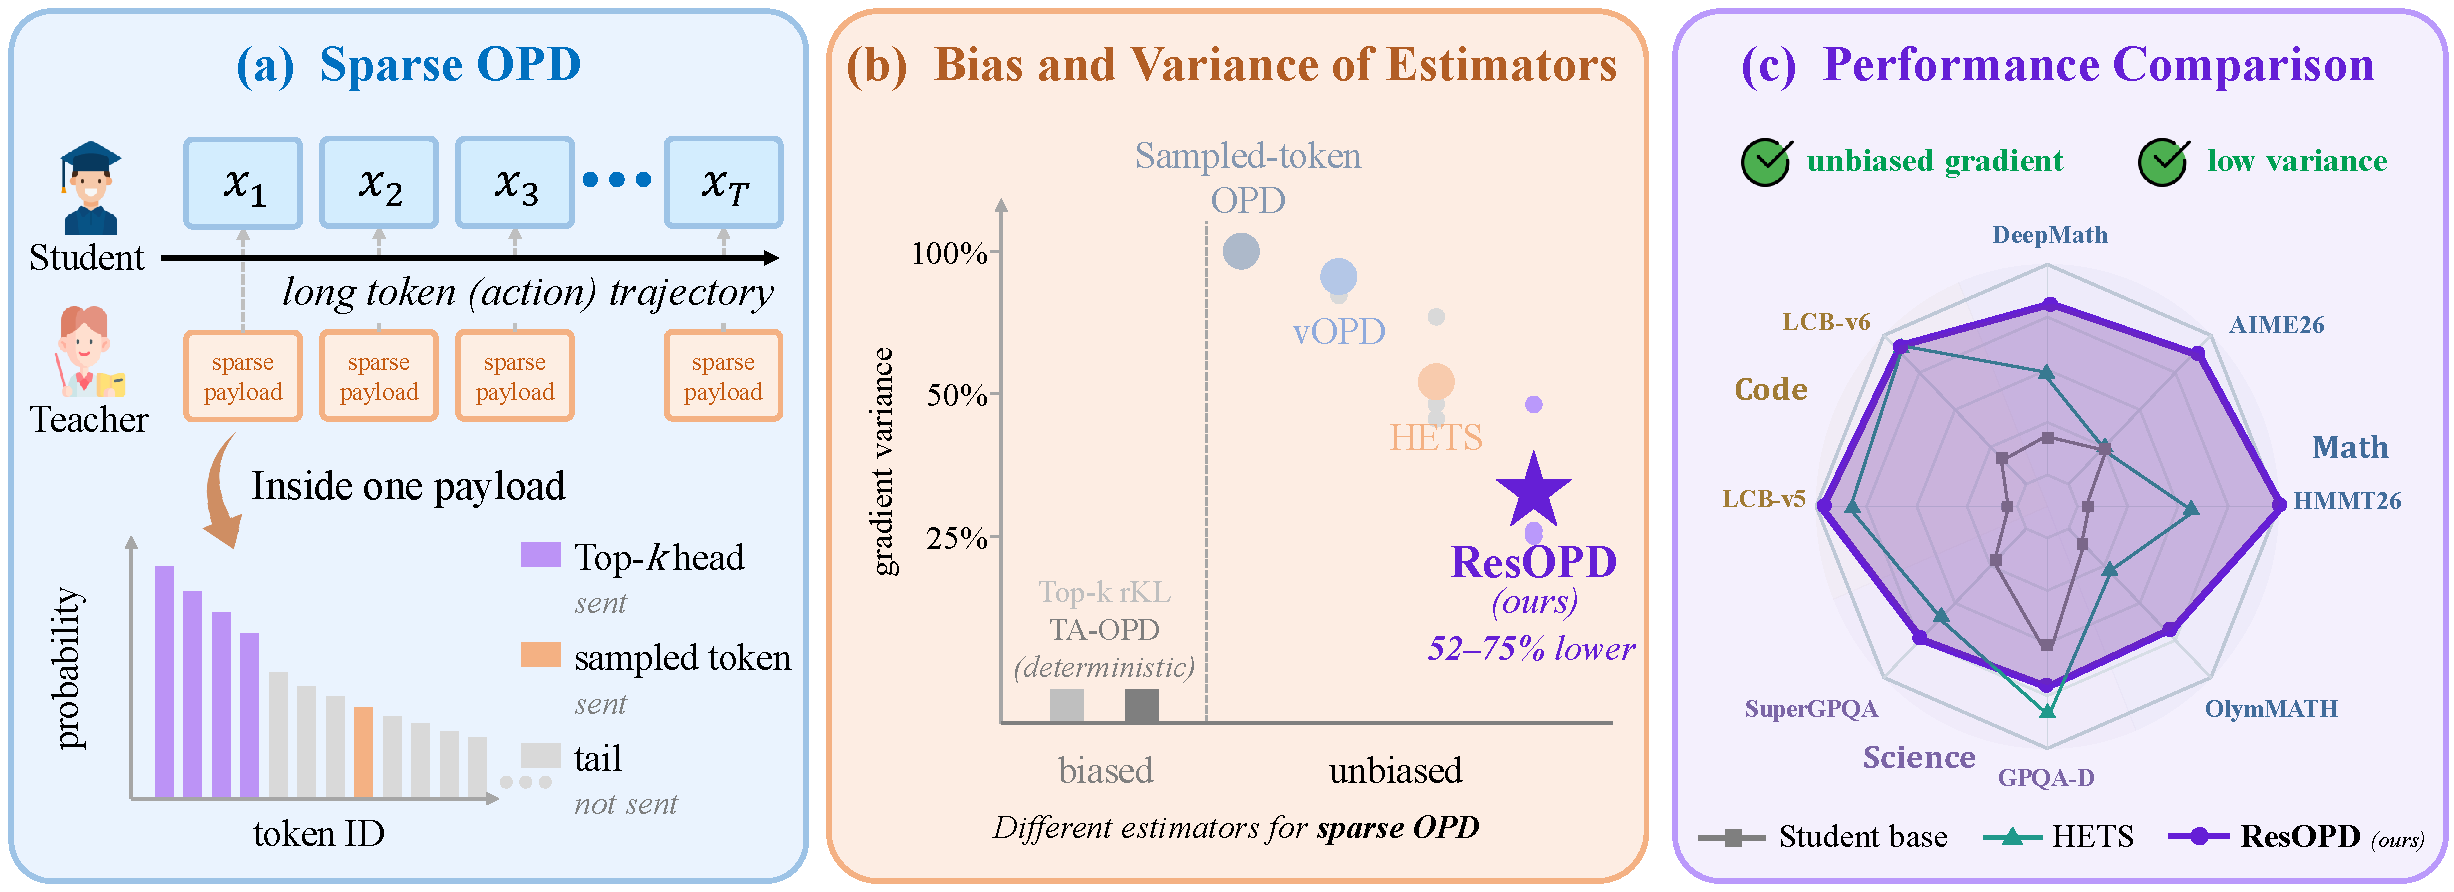
\includegraphics[width=1.0\textwidth]{figs/teaser_v21.pdf}
\caption{(a) 稀疏 OPD：教师模型仅发送 Top-$k$ 头部概率和采样 token 得分，尾部分布未被观测。(b) 偏差 vs. 方差权衡：虽然确定性 Top-$k$ 替代品存在系统性梯度偏差，但 ResOPD 提供了无偏梯度估计量并显著降低了梯度方差。(c) 下游评估：雷达图显示了数学、编程和科学领域的基准得分；尽管相对秩因任务而异，但 ResOPD 实现了最佳整体性能。}
\label{fig:estimator-anatomy}
\vspace{-4mm}
\end{figure}

为解决这一权衡，我们从梯度估计量的角度分析稀疏的OPD。我们首先证明，任何精确评估头部、添加由学生尾部质量加权的前缀相关控制向量，并在尾部命中时进行修正的估计量，对于全词表rKL梯度是无偏的，其中HETS是控制向量为零的特例（第~\ref{subsec:cfr}节）。我们的协方差-迹分解表明，方差分为一个与尾部采样不变的项和一个与控制向量到真实尾部均值距离成比例的事件间项。这解释了HETS的梯度尖峰现象：其零控制在每次命中时都需承担完整的尾部均值代价，而任何能更好预测该均值的控制向量均可严格降低方差。关键的是，头部之外的残差质量定义了一个粗粒度伪token \citep{anshumann-etal-2025-sparse,huang2026tail}，其解析梯度可作为可计算的尾部均值预测器。基于此，我们提出\textit{\textbf{O}n-\textbf{P}olicy \textbf{D}istillation with Tail \textbf{Res}idualization}（ResOPD）：每一步它计算$(k+1)$-路粗粒度分布的精确梯度，仅在尾部命中时添加微小残差修正（图~\ref{fig:framework}(a)）。所得估计量在保持相同稀疏教师负载的同时，被证明是无偏的。

我们在两种情景下评估了 ResOPD。在确切的冻结前缀审计中，通过枚举每个下一个 token 的动作，ResOPD 在 Top-$4$ 反馈下相较于采样 token 的 OPD 降低了 52--75\% 的梯度协方差迹，优于 HETS 和一个与载荷匹配的 vOPD 基准（表~\ref{tab:mechanism}）。在从 Qwen3.5-27B 到 Qwen3.5-4B 的端到端蒸馏中，它在四个数学推理基准上取得了所评估的稀疏 OPD 基准中的最高平均得分，相较于相同载荷下的 HETS 高出 4.40 分（表~\ref{tab:math-terminal}），且其相对于 HETS 的平均优势在所有测试的支持大小 $k\in\{1,4,16,32\}$ 下均保持一致，差距较小（表~\ref{tab:topk-breakdown}）。

我们的贡献如下：  
(1) \textbf{稀疏OPD的有偏与方差分析。} 我们证明了截断、重归一化以及停止系数的Top-$k$  rKL目标函数均为全词表目标函数的有偏替代，我们推导出一种协方差-迹分解，将尾部采样方差与事件间方差分离。该分解给出了粗粒度尾部控制相较于HETS降低方差的确切条件，并提出一个包含两类控制的家族，其中HETS、ResOPD以及同期的SC-TA \citep{huang2026tail} 均可作为特例。  
(2) \textbf{ResOPD估计量。} 我们提出一种估计量，将全词表rKL梯度分解为一个在每一步精确计算的$(k+1)$ -路粗粒度项，该部分基于Top-$k$ 的有效负载和残余尾部质量，以及仅在回放token落入尾部时才应用的尾部内部残差修正。该估计量在同策略采样下无偏，且无需额外的教师查询或前向传播。  
(3) \textbf{实验验证。} 通过确切的冻结前缀梯度审计及端到端蒸馏设置，我们表明ResOPD降低了梯度协方差，减少了训练过程中的在线残差矩，并在下游任务中提升了相对于所评估稀疏OPD基准的准确率。

\section{相关工作}

\paragraph{同策略语言模型蒸馏。}
同策略蒸馏（OPD）通过在稠密教师监督下使用自生成的轨迹进行学生模型训练，缓解了曝光偏差 \citep{gu2024minillm,agarwal2024policy}。后续工作探索了偏斜散度 \citep{ko2024distillm}、自适应目标 \citep{jang2026stable,heo2026policy,jin2026entropy} 以及复杂推理场景中的诊断行为 \citep{fu2026revisiting,zhu2026many}。然而，全词表 OPD 在分布式轨迹生成过程中会产生难以承受的通信和内存开销，严重制约其可扩展性。
\vspace{-4mm}
\paragraph{稀疏散度与截断偏差。}
为缓解通信瓶颈，分布式训练通常采用稀疏的教师端 Top-$k$ 信息包 \citep{zhu2026many}。然而，简单地对 Top-$k$ 支持集进行重归一化或截断，会优化一个有偏的代理目标，导致尾部概率质量分配错误。尽管诸如 TA-OPD \citep{huang2026tail} 等粗支持方法引入了一个虚拟 token \citep{anshumann-etal-2025-sparse} 来聚合被忽略的概率质量，它们仍优化一个代理 $(k+1)$ -way 散度，忽略了教师端尾部内部的细粒度几何结构。
\vspace{-4mm}
\paragraph{随机估计量与方差减小。}
一种替代范式构建了随机估计量，以无偏地恢复真实的全词表 rKL 梯度。标准的采样 token 估计量 \citep{gu2024minillm,lu2025onpolicydistillation} 存在极端的蒙特卡罗方差，促使人们提出如 vOPD \citep{oh2026kl} 这样的方差减少基准方法。HETS 是 EMA-PG \citep{zhang2026ema} 提出的一种混合方案，它对前 $k$ 个 head 进行解析计算，仅在尾部进行采样，但仍在尾部命中时引发严重的梯度突增，导致训练动态不稳定。

\section{方法学}
\label{sec:event}

在本节中，我们介绍了\textit{{O}n-{P}olicy {D}istillation with Tail {Res}idualization}（ResOPD）的理论基础与算法框架。  
我们在第~\ref{subsec:prelim}节中首先建立了全词表逆KL梯度，并分析了稀疏教师输出所引发的权衡问题，揭示了朴素的Top-$k$启发式方法如何导致目标偏差，以及为何混合估计量如HETS会受到尾部采样方差的影响。  
在第~\ref{subsec:cfr}节中，我们提出了ResOPD（如图~\ref{fig:framework}所示），展示了聚合尾部质量如何作为解析控制变量，以实现无偏且方差降低的估计量。  
第~\ref{subsec:evidence}节描述了采样假设，并将理论协方差界与可观测的在线诊断及下游任务性能联系起来。  
最后，第~\ref{sec:unified}节将分析扩展至双控制参数族。



\subsection{预备知识：从采样梯度到精确的稀疏头部}
\label{subsec:prelim}

在某一固定的轨迹前缀下，设 $p(i)>0$  和 $q(i)>0$ 表示学生模型和教师模型在共享词表 $\mathcal V$ 上的下一个 token 概率。定义
\begin{equation}
 \begin{aligned}
 r_i &\coloneqq \log\frac{p_i}{q_i}, &
 \bscore_i &\coloneqq \nabla_\theta\log p_i, &
 \btoken_i &\coloneqq r_i\bscore_i.
 \end{aligned}
 \label{eq:token-gradient}
\end{equation}
由于 $\sum_i p_i\bscore_i=\bm 0$ ，全词表反向KL梯度为
\begin{equation}
 \bgrad
 =\sum_i p_i\btoken_i
 =\E_{A\sim p}\!\left[\btoken_A\right].
 \label{eq:full-gradient}
\end{equation}
此处，$\btoken_A$ 表示停止系数采样 token 的 OPD 梯度。公式~(\ref{eq:full-gradient}) 表明，该采样 token 梯度是全词表反向 KL 梯度的无偏估计量。

\paragraph{为什么直接使用教师模型的 Top-$k$  rKL 会产生有偏结果。}
令 $S$ 为固定的教师 Top-$k$ 支持，其中 $0<k<|\mathcal V|$ ， $P=\sum_{i\in S}p_i$  和
$Q=\sum_{i\in S}q_i$ 。两种常见的标量快捷方式具有不同的偏差：
\begin{equation}
 L_{\mathrm{renormalized}}
 =\KL\!\left(\frac{p_S}{P}\middle\|\frac{q_S}{Q}\right),
 \qquad
 L_{\mathrm{truncated}}=\sum_{i\in S}p_i\log\frac{p_i}{q_i}.
 \label{eq:topk-shortcuts}
\end{equation}
重新规范化仅取决于 $S$ 内的条件分布。并且对于每个省略的 Logit $z_j$ ， $\partial L_{\mathrm{renormalized}}/\partial z_j=0$ 。截断保留了未规范化的头部但引入了一个边界项：
\begin{equation}
 \frac{\partial L_{\mathrm{truncated}}}{\partial z_j}
 =-p_j\underbrace{\sum_{i\in S}p_i(r_i+1)}_{C_S},
 \qquad j\notin S.
 \label{eq:truncated-tail-push}
\end{equation}
当 $C_S>0$ 时，梯度下降会增加每个被省略的 Logit。我们在实验中采用停止系数的替代方法 \citep{zhu2026many} $\bhead=\sum_{i\in S}p_i r_i\bscore_i$，这种方法避免了标量边界项，但仍受省略尾部的影响。附录~\ref{app:topk-bias} 证明了上述三个声明。

\begin{figure}[t]
\centering
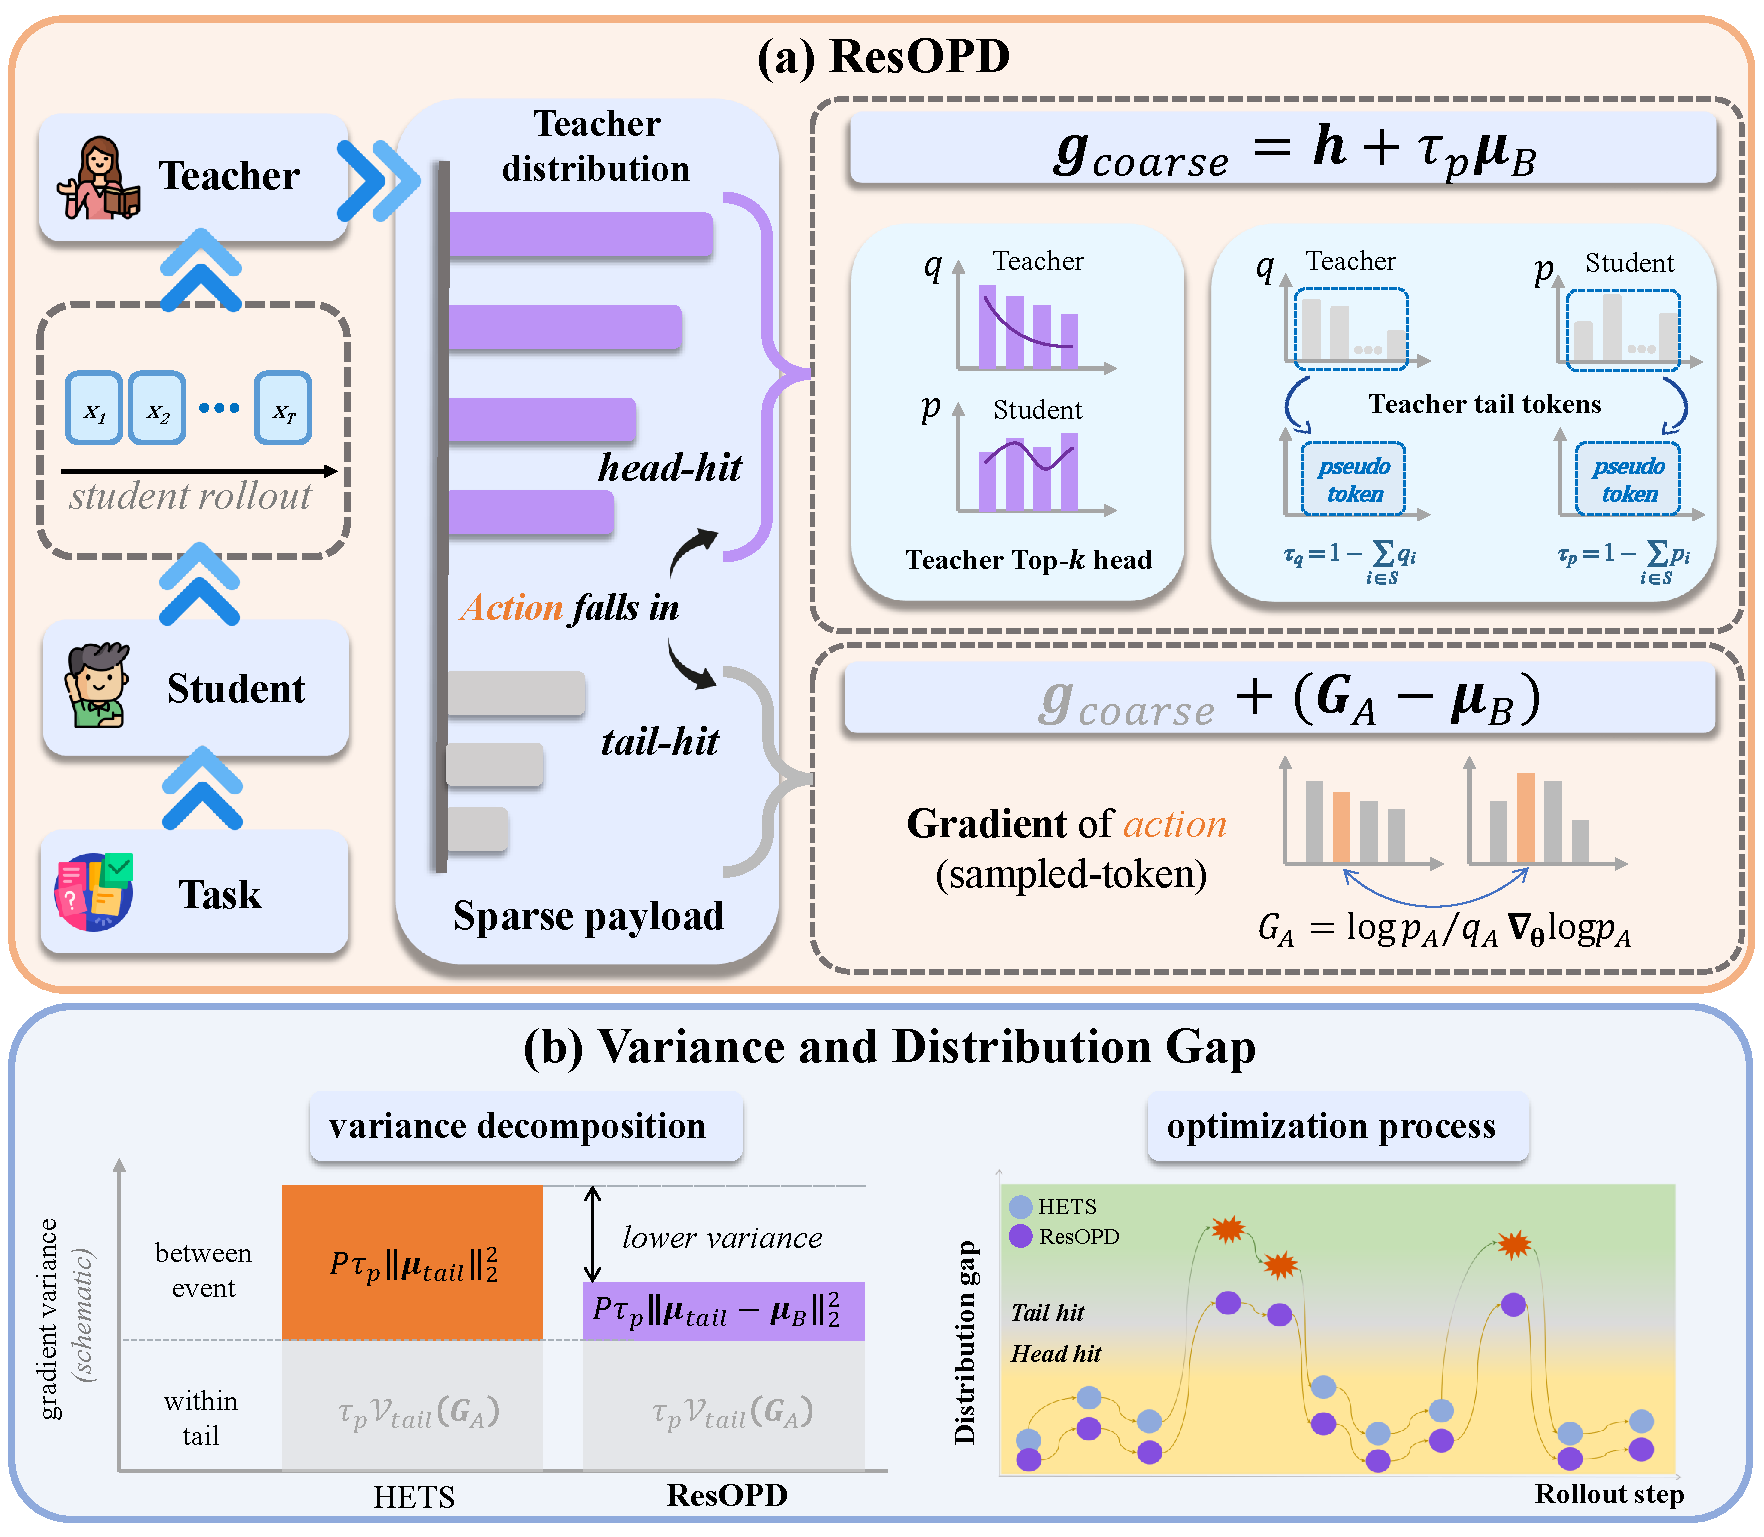
\includegraphics[width=0.8\textwidth]{figs/framework_v11.pdf}
\caption{
\textbf{ResOPD 概述。}
(a) 当学生样本 token 落在头部时，ResOPD 仅使用确切的粗粒度梯度；当命中尾部时，它添加残差修正。(b) 与 HETS 相比，ResOPD 通过将尾部样本集中在 $\boldsymbol{\mu}_B$ 附近，抑制了事件间的方差，从而在轨迹推进步骤中实现了与教师分布更优的对齐。
}
\label{fig:framework}
\end{figure}

接口返回 $q_i$  的完整规范化值以及 $i\in S$  和 $q_A$  的样本动作。
\begin{equation}
  \begin{gathered}
  \tau_p\coloneqq1-P,\qquad \tau_q\coloneqq1-Q,\\[-1pt]
  \bhead\coloneqq P\,\E[\btoken_A\mid A\in S] = \sum_{i\in S} p_i\btoken_i,
  \qquad
  \bmean_{\mathrm{tail}}\coloneqq
  \E\!\left[\btoken_A\mid A\notin S\right] = \frac{1}{\tau_p}\sum_{i\notin S} p_i\btoken_i.
  \end{gathered}
  \label{eq:head-tail-definitions}
\end{equation}
头部 $\bhead$ 是确切已知的，而细尾部平均梯度不可用。使用 $J=\ind\{A\notin S\}$ ，先验的头部确切尾部样本估计量为
\begin{equation}
 \widehat{\bgrad}^{\mathrm{HETS}}
 =\bhead+J\btoken_A,
 \qquad
 \E\!\left[\widehat{\bgrad}^{\mathrm{HETS}}\right]
 =\bhead+\tau_p\bmean_{\mathrm{tail}}=\bgrad.
 \label{eq:g0}
\end{equation}
在头部采样上，这个 \gzero{} 基准 \citep{zhang2026ema} 等于停止的教师 Top-$k$ rKL，并且仅在尾部采样上添加整个修正：
\begin{equation}
 \widehat{\bgrad}^{\mathrm{HETS}}
 =
 \begin{cases}
  \bhead, & A\in S,\\
  \bhead+\btoken_A, & A\notin S,
 \end{cases}
 \qquad
 \Pr(A\in S)=P.
 \label{eq:g0-rare-correction}
\end{equation}
大 $P$ 因此创建了一个稀疏修正模式：大多数 token 使用有偏的仅头部更新，而长小批量仍会累积大量采样的尾部修正。

\subsection{尾部残差化}
\label{subsec:cfr}

Top-$k$  also reveals aggregate tail masses.  
Following the tail-bucketing approach in \citet{hubotter2026reinforcement} and \citet{huang2026tail}, 将尾部合并为一个伪 token 可以得到
\begin{equation}
 \begin{aligned}
 b&\coloneqq\log\frac{\tau_p}{\tau_q}, &
 \bar{\bscore}_{\mathrm{tail}}
 &\coloneqq\E[\bscore_A\mid J=1]
   =\nabla_\theta\log\tau_p, &
 \bmean_B&\coloneqq b\,\bar{\bscore}_{\mathrm{tail}}.
 \end{aligned}
 \label{eq:bucket-vector}
\end{equation}
所得完整粗略分布的确切梯度是
\begin{equation}
 \bgrad_{\mathrm{coarse}}
 =\bhead+\tau_p\bmean_B.
 \label{eq:coarse-gradient}
\end{equation}
此处 $\bmean_B$ 作出预测，但不必等于不可用的细尾均值。事实上，此公式可泛化至任意基准向量：对于 $A\sim p$ 以及任意依赖前缀的基准向量 $\bcontrol$ ，
\begin{equation}
\widehat{\bgrad}(\bcontrol)=\bhead+\tau_p\bcontrol+J(\btoken_A-\bcontrol),
\label{eq:residualization}
\end{equation}
是无偏的，即 $\E_{A\sim p}\!\left[\widehat{\bgrad}(\bcontrol)\right]=\bgrad$ 。图~\ref{fig:framework} 总结了构造过程。HETS 是特殊情况 $\bcontrol=\bm0$ 。期望是显式的：
\begin{equation}
 \E[\widehat{\bgrad}(\bcontrol)]
 =\bhead+\tau_p\bcontrol
  +\tau_p(\bmean_{\mathrm{tail}}-\bcontrol)
 =\bgrad.
 \label{eq:residualization-expectation}
\end{equation}
该控制可能依赖于固定的前缀和当前的模型概率，但必须相对于采样的动作固定，并在反向传播之前停止。此外，将任意随机向量 $\bm{X}$ 的总方差定义为 $\mathcal{V}(\bm{X}) \coloneqq \operatorname{tr}(\operatorname{Cov}(\bm{X}))$，应用全协方差法则可得 $\widehat{\bgrad}(\bm B)$ 的显式方差：
\begin{equation}
\mathcal{V}(\widehat{\bgrad}(\bm B)) = \tau_p\mathcal{V}_{\mathrm{tail}}(\btoken_A)
+ P\tau_p\lVert\bmean_{\mathrm{tail}}-\bm B\rVert_2^2,
\label{eq:single-control-variance-1}
\end{equation}
其中 $\mathcal{V}_{\mathrm{tail}}(\btoken_A) \coloneqq \operatorname{tr}(\operatorname{Cov}(\btoken_A \mid A \in \mathrm{tail}))$。
此处，第一项 $\tau_p\mathcal{V}_{\mathrm{tail}}(\btoken_A)$ 捕捉了尾部采样方差的基准不变性（按尾部概率 $\tau_p$ 加权），而第二项则考虑了由残差近似误差 $\lVert\bmean_{\mathrm{tail}}-\bm B\rVert_2^2$ 引起的事件间方差，该方差通过 \(P\tau_p\)（头部与尾部指示变量的方差）进行缩放。
直接观察可知，对 $J$ 进行条件化：头部分支是确定性的，尾部分支保留 $\Cov_{\mathrm{tail}}(\btoken_A)$，且两者条件均值之差为 $\bmean_{\mathrm{tail}}-\bm B$。根据全协方差定律，得到公式~(\ref{eq:single-control-variance-1})。

公式~(\ref{eq:single-control-variance-1}) 还表明，当控制向量设置为真实的尾部均值时，即 $\bcontrol = \bmean_{\mathrm{tail}}$，估计量 $\widehat{\bgrad}(\bcontrol)$ 的方差达到最小。然而，在实际应用中 $\bmean_{\mathrm{tail}}$ 无法获得，因此 ResOPD 使用可计算的尾部分桶替代量 $\bmean_B$ 来代替它：
\begin{equation}
\widehat{\bgrad}^{\mathrm{ResOPD}}
=\bgrad_{\mathrm{coarse}}+J(\btoken_A-\bmean_B).
\label{eq:event}
\end{equation}

可预测的粗略修正现在每次绘制都会出现；只有细微尾部残差仍然罕见。当 $\lVert\bmean_{\mathrm{tail}}-\bmean_B\rVert_2 < \lVert\bmean_{\mathrm{tail}}\rVert_2$ 时，ResOPD 的方差严格低于 HETS，即当尾部桶向量 $\bmean_B$ 对真实尾部均值的预测优于零时，这在我们冻结前缀审计的总体观察中已得到验证。完整的推导过程见附录~\ref{app:single-control}。





\subsection{采样假设与证据边界}
\label{subsec:evidence}

上述无偏性恒等式假设在固定前缀处 $A\sim p_\theta$。滚动采样过滤器改变了这一采样规律。我们的主要数学实验（第~\ref{sec:math-opd}节）使用温度 $1.0$、滚动 top-$p=0.95$ 和滚动 top-$k=20$，而全支持审计（第~\ref{sec:exact-audit}节）和跨领域实验（第~\ref{sec:cross-domain}节）则采用祖先条件。第~\ref{sec:ex-setup}节同时指定了两者，第~\ref{sec:rollout-ablation}节评估移除过滤器的影响。

粗粒度到细粒度的方差分解也可以在任意实现的滚动分布 $\tilde p$ 下进行刻画。令 $\tilde{\tau}=\Pr_{\tilde p}(A\notin S)$ 和 $\tilde{\bm\mu}_{\mathrm{tail}}
=\mathbb{E}_{\tilde p}[\bm G_A\mid A\notin S]$。对于 $\hat{\bm g}(\bm B)=\bm h+\tau_p\bm B+
\mathbb{I}\{A\notin S\}(\bm G_A-\bm B)$，该估计量仍然具有确切的分解。
\begin{equation}
\mathcal V_{\tilde p}(\hat{\bm g}(\bm B))
=
\tilde{\tau}\mathcal V_{\tilde p,\mathrm{tail}}(\bm G_A)
+
(1-\tilde{\tau})\tilde{\tau}
\|\tilde{\bm\mu}_{\mathrm{tail}}-\bm B\|_2^2 .
\label{eq:realized-rollout-variance}
\end{equation}
因此，对于 $0<\tilde{\tau}<1$ ，当满足 $\|\tilde{\bm\mu}_{\mathrm{tail}}-\bm\mu_B\|_2
<\|\tilde{\bm\mu}_{\mathrm{tail}}\|_2$ 时，ResOPD 的采样方差严格低于 HETS。
在此实现的采样定律下的期望更新为
\begin{equation}
 \E_{\tilde p}[\widehat{\bgrad}(\bm B)]
 =\bhead+\tau_p\bm B
  +\tilde\tau(\tilde{\bm\mu}_{\mathrm{tail}}-\bm B).
 \label{eq:realized-rollout-mean}
\end{equation}
方差恒等式在 $\tilde p$ 下仍然确切成立，但它并不能将截断的滚动序列转化为从 $p_\theta$ 中无偏抽取的样本。  
关键的是，截断严格局限于序列生成过程。在训练期间，所有学生量（$p_i$、$r_i$、$s_i$、$\tau_p$ 以及粗尾项）均通过一次全新的、未截断的前向传播被准确重新计算。

公式~(\ref{eq:single-control-variance-1}) 在固定前缀下刻画了估计量的质量。我们通过确切的动作枚举进行测试（第~\ref{sec:exact-audit}~节）。在在线 OPD 过程中，策略和访问过的前缀均发生变化，而稀疏的教师反馈掩盖了尾部的细微信息。我们转而监控残差的二阶矩 \(M_2\)，作为一种低成本且与机制对齐的在线诊断手段。其下降趋势与头部与尾部事件噪声的减少一致，但本身并不能估计完整的梯度协方差。附录~\ref{app:online-residual-moments} 给出了确切的定义。

然而，方差减小并不意味着下游准确率的单调提升。降低协方差迹可以减少随机优化噪声，但最终性能仍受训练动态和解码随机性的影响，而这两者均通过基准评分进行了离散化。因此，ResOPD能够可靠地抑制梯度噪声，而无需在每个检查点都严格优于HETS。我们因此将理论协方差、在线残差矩以及下游准确率视为学习流水线不同阶段的互补信号。

\FloatBarrier
\subsection{稀疏梯度估计量的统一视角}
\label{sec:unified}

ResOPD 改变了 HETS 方差中的事件间分量，同时保持了其条件下的尾部随机性。这一区别提供了一种有用的方法来比较稀疏无偏估计量：第二个条件均值为零的控制变量可以在尾部内部起作用。本文在此介绍了该族估计量、其最优预言者以及决定 ResOPD--SC-TA 比较的确切条件。相应的审计和下游结果见第~\ref{sec:control-comparison} 节。

\subsubsection{区分事件间与尾部内控制}
\label{sec:joint-family}
\label{sec:event-scta}

单控制族仅作用于头对尾事件分量。第二个控制可以在不改变稀疏教师数据负载的情况下，降低尾部中剩余的条件方差。定义条件零均值得分波动
$\bfluct_A=b(\bscore_A-\bar{\bscore}_{\mathrm{tail}})$ ，使得
$\E[\bfluct_A\mid J=1]=\bm0$ 。对于任意有限前缀可测的 $\bm B$ 以及标量 $\gamma$ ，两者均在抽取 $A$ 之前停止，定义

\begin{equation}
 \widehat{\bgrad}(\bm B,\gamma)
 =\bhead+\tau_p\bm B
 +J\!\left(\btoken_A-\bm B-\gamma\bfluct_A\right).
 \label{eq:unified-main}
\end{equation}
方程~(\ref{eq:unified-main}) 满足
\begin{equation}
 \begin{aligned}
 \E\!\left[\widehat{\bgrad}(\bm B,\gamma)\right]
 &=\bhead+\tau_p\bm B
   +\tau_p(\bmean_{\mathrm{tail}}-\bm B)
   -\gamma\tau_p\E[\bfluct_A\mid J=1]\\
 &=\bhead+\tau_p\bmean_{\mathrm{tail}}
  =\bgrad.
 \end{aligned}
 \label{eq:family-unbiased-proof}
\end{equation}
在头部事件条件下，其值为 $\bhead+\tau_p\bm B$ ，而在尾部事件条件下，其均值为 $\bhead+\tau_p\bm B+\bmean_{\mathrm{tail}}-\bm B$ 。它们的差值为 $\bmean_{\mathrm{tail}}-\bm B$ ，而只有尾部分支保留了条件随机性。因此，全协方差定律给出
\begin{equation}
 \mathcal V\!\left(\widehat{\bgrad}(\bm B,\gamma)\right)
 =\tau_p\mathcal V_{\mathrm{tail}}(\btoken_A-\gamma\bfluct_A)
 +P\tau_p\lVert\bmean_{\mathrm{tail}}-\bm B\rVert_2^2.
 \label{eq:two-level-variance}
\end{equation}
该因子分解证明了两个控制在迹协方差下正交：$\bm B$ 仅改变事件间项，而 $\gamma$ 仅改变尾部内项。我们称方程~(\ref{eq:unified-main}) 为 \emph{统一} 家族：第一个坐标泛化了方程~(\ref{eq:residualization}) 中的单个控制，而第二个坐标则减去一个已知均值为零的尾部内波动。如果 $\mathcal V_{\mathrm{tail}}(\bfluct_A)>0$，它们的联合虚设模型是
\begin{equation}
 \bm B^\star=\bmean_{\mathrm{tail}},\qquad
 \gamma^\star=
 \frac{\operatorname{tr}\!\left(
       \Cov_{\mathrm{tail}}(\btoken_A,\bfluct_A)\right)}
      {\mathcal V_{\mathrm{tail}}(\bfluct_A)},
 \label{eq:joint-oracle}
\end{equation}
对两个坐标进行配方运算后得到
\begin{equation}
 \begin{aligned}
 &\mathcal V\!\left(\widehat{\bgrad}(\bm B,\gamma)\right)
 -\mathcal V\!\left(
   \widehat{\bgrad}(\bm B^\star,\gamma^\star)\right)\\
 &\qquad
 =P\tau_p\lVert\bm B-\bmean_{\mathrm{tail}}\rVert_2^2
 +\tau_p\mathcal V_{\mathrm{tail}}(\bfluct_A)
  (\gamma-\gamma^\star)^2.
 \end{aligned}
 \label{eq:unified-regret-main}
\end{equation}
如果 $\mathcal V_{\mathrm{tail}}(\bfluct_A)=0$、$\gamma$ 无关紧要，第一项保持确切。重要的是，两种预言坐标均无法在线获得：$\bm B^\star$ 需要完整的教师尾部，而每个前缀的 $\gamma^\star$ 需要其条件协方差。ResOPD 则采取了简单但有效的选择 $(\bmean_B,0)$，全局拟合系数是一个分离的离线诊断。

\begin{table}[t]
\caption{双控制族中的坐标。}
\label{tab:estimator-map}
\centering
\begin{tabular*}{0.7\linewidth}{@{\extracolsep{\fill}} lccc @{}}
\toprule
Unbiased estimator & $\bm B$ & $\gamma$ & Role \\
\midrule
HETS & $\bm 0$ & $0$ & structural baseline \\
ResOPD & $\bmean_B$ & $0$ & our estimator \\
SC-TA & $\bmean_B$ & $1$ & boundary estimator \\
Joint oracle & $\bmean_{\mathrm{tail}}$ & $\gamma^\star$ & unavailable optimum \\
\bottomrule
\end{tabular*}
\end{table}
\subsubsection{ResOPD和SC-TA作为主要终点}
\label{sec:gamma}

我们现在将两层族特化为 $\bm B=\bmean_B$，并将其与 \citet{huang2026tail} 的同期工作中提出的样本修正型 TA-OPD（SC-TA）联系起来。其主要方法 TA-OPD 通过引入尾部伪 token 来增强教师 Top-$k$ 支持，优化由此产生的粗粒度 $(k+1)$ -way 反向 KL 目标。随后，SC-TA 被推导为一种恢复完整词表无偏性的样本修正变体。我们在此基础上，通过我们两控制族内的梯度层面刻画加以补充。具体而言，我们推导出 ResOPD 与 SC-TA 之间的确切逐点关系，将它们的协方差排序表征为尾部内控制系数 $\gamma$ 的函数，识别出迹最优的 $\gamma^\star$ ，并在自然提示分布上评估了这些预测。

\paragraph{确切的精细分解。}
在尾部拉伸时，
\begin{equation}
 r_A
 =\log\frac{p_A}{q_A}
 =\underbrace{\log\frac{\tau_p}{\tau_q}}_{b}
 +\log\frac{p_A/\tau_p}{q_A/\tau_q}.
\end{equation}
使用 $\bmean_B=b\bar{\bscore}_{\mathrm{tail}}$  因此得到
\begin{equation}
 \btoken_A
 =\bmean_B
 +\underbrace{b(\bscore_A-\bar{\bscore}_{\mathrm{tail}})}_{\bfluct_A}
 +\underbrace{(r_A-b)\bscore_A}_{\bresid_A},
 \qquad
 \E[\bfluct_A\mid J=1]=\bm 0.
 \label{eq:tail-exact-decomposition}
\end{equation}
这些术语具有不同的作用。$\bmean_B$ 是粗粒度尾部桶预测；$\bfluct_A$ 是围绕条件学生得分的已知零均值波动；$\bresid_A$ 记录了未解析的学生-教师条件尾部形状不匹配。

使用 $\bgrad_{\mathrm{coarse}}=\bhead+\tau_p\bmean_B$，方程~(\ref{eq:unified-main}) 的特化为
\begin{equation}
 \widehat{\bgrad}_\gamma
 =\bgrad_{\mathrm{coarse}}
 +J\!\left[\bresid_A+(1-\gamma)\bfluct_A\right].
 \label{eq:event-scta-family}
\end{equation}
公式~(\ref{eq:family-unbiased-proof}) 已经证明了每个固定的 $\gamma$ 都会指向 $\bgrad$。它的两个命名端点是
\begin{equation}
 \begin{aligned}
 \widehat{\bgrad}^{\mathrm{ResOPD}}
 &=\widehat{\bgrad}_{\gamma=0}
  =\bgrad_{\mathrm{coarse}}+J(\bresid_A+\bfluct_A),\\
 \widehat{\bgrad}^{\mathrm{SC}}
 &=\widehat{\bgrad}_{\gamma=1}
  =\bgrad_{\mathrm{coarse}}+J\bresid_A.
 \end{aligned}
\end{equation}
因此，它们的带符号点态关系是
\begin{equation}
 \boxed{
 \widehat{\bgrad}^{\mathrm{SC}}
 =\widehat{\bgrad}^{\mathrm{ResOPD}}-J\bfluct_A
 }
 \label{eq:event-scta-difference}
\end{equation}
该差异的期望值为零，但在尾部动作上通常不为零。

\paragraph{方差最优与端点证书。}
令 $\bz_0 = \bresid_A + \bfluct_A = \btoken_A - \bmean_B$。将总方差分解为事件间共同成分和与 $\gamma$ 有关的尾部内成分，可得
\begin{equation}
  \begin{aligned}
    \mathcal{V}(\widehat{\bgrad}_\gamma)
    &= \tau_p \mathcal{V}_{\mathrm{tail}}(\bz_0 - \gamma \bfluct_A) + P\tau_p \lVert\bmean_{\mathrm{tail}} - \bmean_B\rVert_2^2, \\
    \mathcal{V}_{\mathrm{tail}}(\bz_0 - \gamma \bfluct_A)
    &= \mathcal{V}_{\mathrm{tail}}(\bz_0) - 2\gamma \operatorname{tr}\!\left(\Cov_{\mathrm{tail}}(\bz_0, \bfluct_A)\right) + \gamma^2 \mathcal{V}_{\mathrm{tail}}(\bfluct_A).
  \end{aligned}
  \label{eq:event-scta-total-var}
\end{equation}
当 $\mathcal{V}_{\mathrm{tail}}(\bfluct_A) > 0$ 时，对 $\gamma$ 进行配方可确定迹的最优值：
\begin{equation}
  \begin{aligned}
    \gamma^\star
    &= \frac{\operatorname{tr}\!\left(\Cov_{\mathrm{tail}}(\bz_0, \bfluct_A)\right)}{\mathcal{V}_{\mathrm{tail}}(\bfluct_A)}, \\
    \mathcal{V}(\widehat{\bgrad}_\gamma) - \mathcal{V}(\widehat{\bgrad}_{\gamma^\star})
    &= \tau_p \mathcal{V}_{\mathrm{tail}}(\bfluct_A) (\gamma - \gamma^\star)^2.
  \end{aligned}
  \label{eq:event-scta-regret}
\end{equation}
在边界点 $\gamma = 1$（SC-TA）和 $\gamma = 0$（ResOPD）处评估二次损失，可发现当且仅当 $\gamma^\star > 1/2$ 时，SC-TA 的迹协方差严格低于 ResOPD。将 $\bz_0 = \bresid_A + \bfluct_A$ 代入后，最优系数展开为
\begin{equation}
  \gamma^\star = 1 + \frac{\operatorname{tr}\!\left(\Cov_{\mathrm{tail}}(\bresid_A, \bfluct_A)\right)}{\mathcal{V}_{\mathrm{tail}}(\bfluct_A)}.
  \label{eq:event-scta-gamma-residual}
\end{equation}
因此，当 $\operatorname{tr}\!\left(\Cov_{\mathrm{tail}}(\bresid_A, \bfluct_A)\right) > -\mathcal{V}_{\mathrm{tail}}(\bfluct_A)/2$ 时，SC-TA 的性能优于 ResOPD。根据柯西-施瓦茨不等式，一个充分条件是
\begin{equation}
  \mathcal{V}_{\mathrm{tail}}(\bresid_A) < \mathcal{V}_{\mathrm{tail}}(\bfluct_A)/4.
  \label{eq:event-improvement}
\end{equation}
特别是，当条件尾部形状匹配时，残差消失（$\bresid_A = \bm{0}$），从而得到 $\gamma^\star = 1$。这些条件作为依赖于分布的凭证，而非保证普遍的方差排序。

\FloatBarrier
\section{实验}
\label{sec:experiments}

我们评估三个互补性问题：残差化是否降低确切条件梯度协方差，其可观测效应在在线训练过程中是否持续存在，以及由此产生的策略是否提升下游性能。我们首先明确实验协议，随后展示冻结前缀审计、数学结果与诊断分析、跨领域迁移，以及对支持集大小、回溯采样、学习率和尾部内控制的受控消融实验。

\subsection{实验设置}
\label{sec:ex-setup}

\paragraph{离线机制审计。}
我们冻结 Qwen3.5 \citep{qwen3.5} 模型，在选定的冻结数学前缀下，每个提示采样一条 64-token 轨迹，测量协方差迹和信噪比：
NSR=$\frac{\mathcal{V}(\hat{\bgrad})}{\|\bgrad_{\text{full-rKL}}\|_2^2}$ 。实验涵盖五种情景：GSM8K \citep{cobbe2021gsm8k}（32 个提示）在 0.8B/4B、4B/27B 和 9B/27B 组合中；全部 33 个 HMMT26 提示 \citep{dekoninck2026matharena}（4B/27B）；以及从 DeepMath-103K \citep{deepmath} 中采样的 64 个提示（4B/27B）。

\paragraph{在线门诊训练数学推理。}
我们从Qwen3.5-27B教师模型中蒸馏出具备思考能力的Qwen3.5-4B学生模型。从DeepMath-103K出发，我们在去重和基准污染移除后筛选出具有挑战性的竞赛问题。为确保适当的师生能力差距，我们保留教师模型在采样生成中成功两次而学生模型至少失败一次的提示。这产生了1,276个独特问题，划分为1,024个用于训练和252个用于条件性留出评估。训练运行3个轮次（192步），在第6、32、64、128和192步保存中间检查点。
\vspace{-4mm}

\paragraph{评估。}
我们的评估涵盖四个基准：DeepMath 留出集、AIME26（30 道题）\citep{aime26}、HMMT26（33 道题）\citep{dekoninck2026matharena}，以及 OlymMATH 的英文划分（200 道题）\citep{sun2025challengingboundariesreasoningolympiadlevel}。由于 AIME26 和 HMMT26 的题目数量有限，我们对每道题报告 16 次采样响应的平均值（avg@16）以缓解评估方差，而 DeepMath 留出集和 OlymMATH 使用 avg@2。除了最终性能外，我们还评估所有中间保存的检查点，以计算曲线下面积（AUC），量化学习动态和训练效率。我们在保存的检查点轨迹上计算规范化的梯形 AUC，并对每个基准的得分和 AUC 进行平均，得到汇总列。训练与评估的完整配置详见附录~\ref{app:hyperparameters}。
\vspace{-4mm}

\paragraph{实现的滚动分布。}
根据 Qwen3.5 官方配方，主要的数学推理和评估使用温度 $1.0$、top-$p=0.95$ 和 top-$k=20$。  
截断低概率 token 有助于避免导致 OPD 和教师反馈~\citep{fu2026revisiting} 不稳定的退化前缀。  
训练中使用的学生端概率通过一次全新的、未截断的前向传播重新计算。如第~\ref{subsec:evidence} 节所述，这种设置保持了明确的采样方差对比，但不满足理想化的全 rKL 无偏假设。  
因此，我们还报告了一个匹配的全支持数学消融实验（第~\ref{sec:rollout-ablation} 节）以及使用 top-$p=1.0$、top-$k=-1$ 的跨领域训练（第~\ref{sec:cross-domain} 节）。


\subsection{确切的冻结前缀协方差审计}
\label{sec:exact-audit}

\begin{table}[t]
\caption{
确切的冻结前缀协方差迹和NSR。学生Logit梯度的协方差迹通过完整动作枚举计算，并在轨迹间取平均；NSR将每个迹除以全-rKL梯度的平方$L_2$范数进行归一化。稀疏估计量($\text{vOPD}_{\text{T-Top-}k}$, HETS, ResOPD) 共享一个相同的教师预算$k=4$，其中$\text{vOPD}_{\text{T-Top-}k}$ 在此支持集上采用分离的条件-KL基准。每行最佳结果用\textbf{粗体}表示，次佳结果用\underline{下划线}表示。
}
\label{tab:mechanism}
\centering
\small
\setlength{\tabcolsep}{2.8pt}
\renewcommand{\arraystretch}{1.18}

\begin{tabular*}{\linewidth}{@{\extracolsep{\fill}}ll cccc cccc@{}}
\toprule
\multirow{2}{*}{\textbf{Dataset}}
& \multirow{2}{*}{\textbf{Models}}
& \multicolumn{4}{c}{\textbf{Covariance Trace} $\downarrow$}
& \multicolumn{4}{c}{\textbf{NSR} $\downarrow$} \\
\cmidrule(lr){3-6} \cmidrule(l){7-10}
&
& \shortstack{Sampled} & \shortstack{$\text{vOPD}_{\text{T-Top-}k}$} & \shortstack{HETS} & \shortstack{ResOPD}
& \shortstack{Sampled} & \shortstack{$\text{vOPD}_{\text{T-Top-}k}$} & \shortstack{HETS} & \shortstack{ResOPD} \\
\midrule
GSM8K    & 0.8B\,/\,4B  & 2.146 & 1.730 & \underline{1.559} & \textbf{1.018} & 5.422 & 4.370 & \underline{3.940} & \textbf{2.573} \\
GSM8K    & 9B\,/\,27B   & 0.215 & 0.192 & \underline{0.107} & \textbf{0.068} & 6.202 & 5.560 & \underline{3.101} & \textbf{1.955} \\
GSM8K    & 4B\,/\,27B   & 0.333 & 0.297 & \underline{0.183} & \textbf{0.108} & 6.058 & 5.400 & \underline{3.335} & \textbf{1.964} \\
HMMT26   & 4B\,/\,27B   & 0.208 & 0.189 & \underline{0.092} & \textbf{0.052} & 6.589 & 5.977 & \underline{2.914} & \textbf{1.630} \\
DeepMath & 4B\,/\,27B   & 0.183 & 0.169 & \underline{0.087} & \textbf{0.047} & 7.352 & 6.785 & \underline{3.500} & \textbf{1.907} \\
\bottomrule
\end{tabular*}
\end{table}

表~\ref{tab:mechanism} 报告了五个冻结前缀面板中的确切协方差迹和NSR。通过在每个学生访问的前缀处解析枚举每一个下一个token的动作，我们隔离了每个估计量的条件采样方差，而不受解码噪声或优化器反馈的影响。在表格中使用的面板级聚合下，这两个指标在每个面板中均表现出一致的排序：$\text{ResOPD} < \text{HETS} < \text{vOPD} < \text{sampled-token OPD}$（越低越好）。相对于采样token的OPD，整体协方差迹在payload匹配的Teacher-Top-$k$ vOPD中减少了$7.7\%\text{--}19.4\%$，\gzero{}中减少了$27.3\%\text{--}55.8\%$，ResOPD中减少了$52.5\%\text{--}75.0\%$。

尽管教师-顶端-$k$ vOPD 在我们的端到端实验中作为具有竞争力的基准（表~\ref{tab:math-terminal}），但其分离的标量控制无法利用结构化的头--尾分解，导致每一步都对整个动作向量进行采样。因此，与 HETS 和 ResOPD 相比，其方差减小效果仍然有限。由于 HETS 和 ResOPD 具有相同的负载预算、确切的前四名头集成以及条件目标结构，它们之间的对比能够直接隔离粗尾残差化带来的增益，而不受基准干扰。因此，我们主要关注从 HETS 到 ResOPD 的演进过程。

随着支持大小 $k$ 增加，确切的 Top-$k$ 头吸收了更多的概率质量，导致剩余尾部机会 $P\tau_p$ 缩小。相应地，ResOPD 相对于 \gzero{} 的边际协方差减小逐渐变窄。附录~\ref{app:fixed-prefix-sweep} 中的完整支持大小扫描直接测试了这种通信--方差权衡。

\subsection{端到端的数学推理}
\label{sec:math-opd}

\begin{table}[t]
\caption{
Qwen3.5-27B-to-4B OPD结果。DeepMath的保留测试集和OlymMATH使用avg@2进行评估，而AIME26和HMMT26由于题目数量较少，采用avg@16进行评估。
}
\label{tab:math-terminal}
\centering
\small
\setlength{\tabcolsep}{3.5pt}
\renewcommand{\arraystretch}{1.18}

\newcolumntype{Y}{>{\centering\arraybackslash}X}

\begin{tabularx}{\linewidth}{l YYYYY Y}
\toprule
\multirow{2}{*}[-2ex]{\textbf{Method}}
& \multicolumn{4}{c}{\textbf{Benchmark Accuracy (\%)}}
& \multicolumn{2}{c}{\textbf{Aggregate (\%)}} \\
\cmidrule(lr){2-5} \cmidrule(l){6-7}
& \shortstack{DeepMath\\{\scriptsize held-out (avg@2)}}
& \shortstack{AIME26\\{\scriptsize(avg@16)}}
& \shortstack{HMMT26\\{\scriptsize(avg@16)}}
& \shortstack{OlymMATH\\{\scriptsize(avg@2)}}
& \shortstack{Avg.\\Score}
& \shortstack{Avg.\\AUC} \\
\midrule

\rowcolor{gray!18}\multicolumn{7}{@{}l}{\textit{\textbf{$\blacktriangledown$ Original Models}}} \\
Qwen3.5-4B Student   & 48.41 & 56.25 & 35.23 & 31.50 & 42.85 & -- \\
Qwen3.5-27B Teacher  & 89.29 & 80.62 & 62.88 & 63.25 & 74.01 & -- \\

\midrule
\rowcolor{gray!18}\multicolumn{7}{@{}l}{\textit{\textbf{$\blacktriangledown$ Alternative Sparse OPD (Biased)}}} \\
Teacher Top-$k$ fKL  & 50.20 & 54.58 & 35.04 & 34.50 & 43.58 & 42.80 \\
Teacher Top-$k$ rKL  & 51.79 & 55.83 & 34.66 & 36.75 & 44.76 & 44.63 \\
TA-OPD               & 58.13 & 58.96 & \underline{39.58} & 36.00 & 48.17 & \underline{47.94} \\

\midrule
\rowcolor{gray!18}\multicolumn{7}{@{}l}{\textit{\textbf{$\blacktriangledown$ Unbiased rKL Estimators}}} \\
Sampled-token OPD    & 48.21 & 57.50 & 36.17 & 34.25 & 44.03 & 46.69 \\
vOPD$_{\text{T-Top-}k}$ & \underline{58.93} & \textbf{60.00} & 39.20 & \underline{37.25} & \underline{48.85} & 47.49 \\
\gzero{}             & 54.76 & 56.25 & 37.88 & 34.00 & 45.72 & 46.18 \\

\rowcolor{lineblue!15}
\textbf{\method{}} (\textit{ours}) & \textbf{60.91} & \underline{59.38} & \textbf{39.96} & \textbf{40.25} & \textbf{50.12} & \textbf{47.96} \\
\bottomrule
\end{tabularx}
\end{table}

表~\ref{tab:math-terminal} 报告了主要的蒸馏结果：在所有评估的OPD基准中，ResOPD实现了最强的综合性能，达到了最高的终端平均得分（50.12\%）和学习轨迹AUC（47.96\%）。这种有利的训练轨迹也延伸至外部数学竞赛。在AIME26、HMMT26和OlymMATH中，其他竞争基准在训练后期表现出明显的峰值后退化，而ResOPD则避免了严重的后期退化，并在最终检查点恢复到其最佳综合性能。中间检查点的分步评估结果在附录~\ref{app:math-learning-trajectories} 中提供并进行了分析。

\subsubsection{训练动态}
\label{sec:train_dynamics}

\begin{table}[t]
\centering
\small
\caption{\textbf{训练过程中的聚合在线诊断}（越低越好）。数值表示所有192个最优化步骤的平均值。$\Delta$ 表示相对于HETS，ResOPD的相对降低百分比。}
\label{tab:stable-dynamics}
\renewcommand{\arraystretch}{1.18}
\setlength{\tabcolsep}{6pt}
\begin{tabular}{lccccc}
\toprule
\textbf{Diagnostic Metric} & \textbf{Top-$k$ rKL} & \textbf{$\text{vOPD}_{\text{T-Top-}k}$} & \textbf{HETS} & \textbf{ResOPD (\textit{ours})} & \textbf{$\Delta$ (\%)$\downarrow$} \\
\midrule
Support-mass gap ($\times10^{-3}$)          & 11.17 & 3.53  & 5.17  & \textbf{3.50}  & $-32.3\%$ \\
$|$Tail log-mass mismatch$|$                 & 0.715 & 0.858 & 0.723 & \textbf{0.322} & $-55.5\%$ \\
Token residual $M_2$ ($\times10^{-3}$)      & --    & \textbf{10.55} & 11.73 & {10.67} & $-9.0\%$  \\
Trajectory residual $M_2$ ($\times10^{-5}$) & --    & 2.76  & 3.50  & \textbf{2.65}  & $-24.3\%$ \\
\bottomrule
\end{tabular}
\vspace{-3mm}
\end{table}

\begin{figure}[t]
\centering
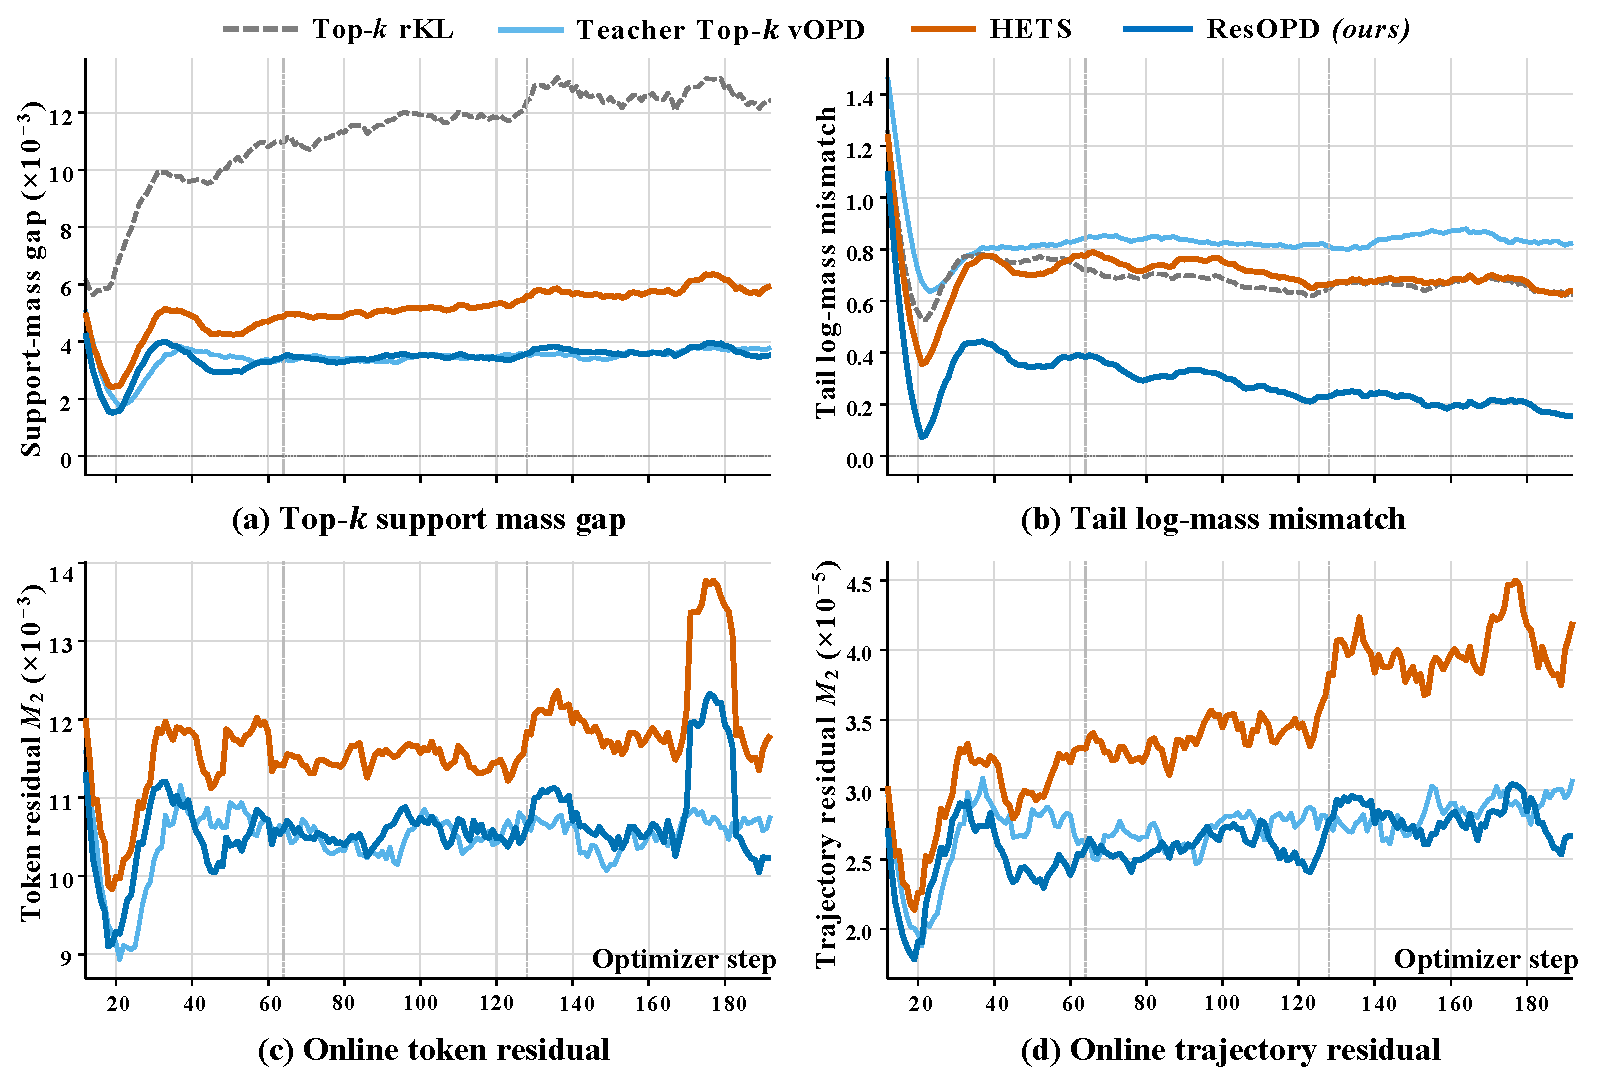
\includegraphics[width=0.85\textwidth]{figs/math_dynamics_v10.pdf}
\caption{\textbf{训练时诊断}（64步/轮次；越低越好）。
\textbf{子图(a)和(b)}展示了在vOPD、HETS、ResOPD和直接教师Top-$k$ rKL中，学生--教师不匹配在Top-$k$支撑质量和尾部对数质量上的情况。
\textbf{子图(c)和(d)}分别通过二值Top-$k$指示器与其学生预测概率之间的平方残差，在token级别和轨迹级别上比较vOPD、HETS和ResOPD。详细公式见附录~\ref{app:online-residual-moments}。}
\label{fig:training-dynamics-event-g0}
\vspace{-6mm}
\end{figure}

如表~\ref{tab:stable-dynamics} 和图~\ref{fig:training-dynamics-event-g0} 所示，与 HETS 相比，ResOPD 在平均 192 个训练步骤中持续抑制了学生-教师质量差异以及随机残差波动。在匹配的 HETS--ResOPD 运行中，ResOPD 将支持质量差距减少了 $32.3\%$ ，并将尾部对数质量不匹配减少了 $55.5\%$ 。尽管 Teacher-Top-$k$ vOPD 展现了相当的支持事件 $M_2$ ，但其在自生成轨迹上的标量残差忽略了中心化对数比和得分几何结构，且在共享冻结前缀上的确切梯度协方差比较（表~\ref{tab:mechanism}）确认了 ResOPD 的结构优势。

这为ResOPD的最优化行为提供了机制性解释。在HETS下，完整的微调尾部梯度修正集中在稀有尾部命中事件上。尽管头部覆盖度约为$98.4\%$，一个$30\text{K}$-token推理迹中仍包含460–470次此类修正，每轮优化器步骤累积达数千次。通过减去可用载荷的尾部桶分量$\bmean_B$，ResOPD在保留同策略条件下第Sec.~\ref{subsec:evidence}中全-rKL期望的同时，重新分配了事件间的可预测成分。下游准确率仍然存在更多噪声，因为它依赖于离散答案的正确性，但仅完成情况的教师NLL审计显示，ResOPD生成的学生轨迹具有更一致更高的教师似然。结合匹配的终点与曲线-AUC结果，这些诊断将估计量层面的协方差减小与更平滑的最优化路径及改进的下游性能联系起来。

\vspace{-4mm}
\subsubsection{行为忠实性}
\label{sec:math-eval-diagnostics}

除了特定任务的准确率指标（例如在下游数学基准上的avg@2和avg@16），监控学生模型在教师模型下的负对数似然值，可以提供一种内在的、与任务无关的蒸馏保真度读数。具体而言，教师模型的较低负对数似然值表明学生样本在教师模型下的似然值更高。

图~\ref{fig:teacher-nll} 跟踪了该度量在匹配的数学运行过程中的变化。如面板~A所示，尽管两种估计量初始值均约为 $0.46$ \,nats/token，但ResOPD在第6步时下降更为迅速，并持续保持单调下降趋势，至第192步时降至 $0.36$ \,nats/token。相比之下，HETS在约 $0.385$ \,nats/token 处趋于平稳，并在后期表现出轻微漂移。在面板~B中，二者之差 $\Delta\text{Teacher-NLL (ResOPD} - \text{HETS)}$ 在所有优化器步骤中始终保持负值，并扩大至超过 $-0.027$ \,nats/token。这表明ResOPD始终比HETS更有效地保持与教师模型的行为一致性，提供了更高教师相似性的证据，与准确率形成互补。


\subsection{跨领域迁移至科学与编程}
\label{sec:cross-domain}

\begin{figure}[htbp]
\centering
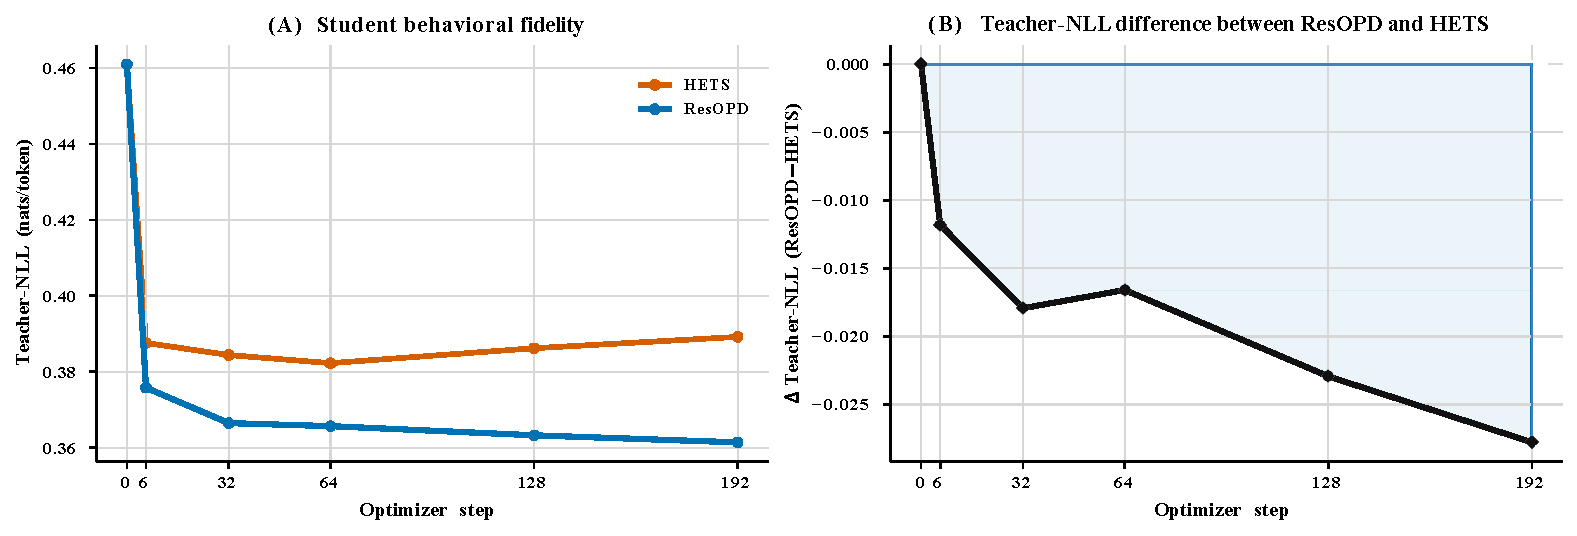
\includegraphics[width=0.9\textwidth]{figs/teacher_nll_fidelity_v3.pdf}
\vspace{-2mm}
\caption{\textbf{Math OPD 设置下训练过程中教师的负对数似然（NLL）}。  
评估在四个核心基准族上进行，权重与主套件相同：AIME26、HMMT26、DeepMath 留出集和 OlymMATH。数值越低，表示对教师分布的保真度越高。}
\label{fig:teacher-nll}
\end{figure}

\begin{table}[h]
\caption{
Qwen3-30B-A3B-Instruct到Qwen3-4B的蒸馏结果。评估使用GPQA-D的avg@10，以及SuperGPQA、LCB-v5和LCB-v6的avg@3。AUC综合了固定训练轨迹（Base/10/25/50/100）上的性能表现。
}
\label{tab:qwen3-transfer}
\centering
\small
\setlength{\tabcolsep}{3.5pt}
\renewcommand{\arraystretch}{1.18}

\newcolumntype{Y}{>{\centering\arraybackslash}X}

\begin{tabularx}{\linewidth}{l YYYY YY}
\toprule
\multirow{2}{*}[-2ex]{\textbf{Method}}
& \multicolumn{2}{c}{\textbf{Science Benchmarks (\%)}}
& \multicolumn{2}{c}{\textbf{Code Benchmarks (\%)}}
& \multicolumn{2}{c}{\textbf{Aggregate (\%)}} \\
\cmidrule(lr){2-3} \cmidrule(lr){4-5} \cmidrule(l){6-7}
& \shortstack{GPQA-D\\{\scriptsize(avg@10)}}
& \shortstack{SuperGPQA\\{\scriptsize(avg@3)}}
& \shortstack{LCB-v5\\{\scriptsize(avg@3)}}
& \shortstack{LCB-v6\\{\scriptsize(avg@3)}}
& \shortstack{Avg.\\Score}
& \shortstack{Avg.\\AUC} \\
\midrule

\rowcolor{gray!18}\multicolumn{7}{@{}l}{\textit{\textbf{$\blacktriangledown$ Original Models}}} \\
Student             & 45.25          & 32.46          & 21.76          & 24.38          & 30.96          & -- \\
Teacher             & 56.06          & 48.87          & 45.51          & 41.71          & 48.04          & -- \\

\midrule
\rowcolor{gray!18}\multicolumn{7}{@{}l}{\textit{\textbf{$\blacktriangledown$ Unbiased rKL Estimators}}} \\
Sampled-token OPD   & \textbf{50.30} & \underline{36.87} & 43.31          & 39.43          & 42.48          & 41.21 \\
HETS                & \underline{48.89} & 36.10          & \underline{46.31} & \textbf{43.24} & \underline{43.63} & \underline{42.13} \\

\rowcolor{lineblue!15}
\textbf{ResOPD} (\textit{ours}) & 47.12          & \textbf{37.54} & \textbf{48.90} & \underline{43.05} & \textbf{44.15} & \textbf{42.65} \\
\bottomrule
\end{tabularx}
\end{table}

为了进一步评估 ResOPD 的泛化能力与跨领域有效性，我们遵循 \citet{heo2026policy} 并将研究范围扩展至科学和编程任务。我们的实验协议在很大程度上模仿了 \citet{heo2026policy}：从一个 Qwen3-30B-A3B-Instruct \citep{yang2025qwen3} 教师模型中蒸馏出一个 Qwen3-4B 学生模型，训练数据为由 OpenMathReasoning \citep{moshkov2025aimo}、OpenScienceReasoning-2 \citep{nvidia2025opensciencereasoning2} 和 OpenCodeReasoning \citep{ahmad2025opencodereasoning} 构成的 30k 样本混合数据集。运行过程中采用全支持的祖先回溯（ancestral rollouts），温度 $1.0$，top-$p=1.0$ 和 top-$k=-1$，不启用思考模式。在评估方面，我们在代码领域上基于 LiveCodeBench \citep[LCB;][]{jain2025livecodebench} v5（167 个问题）和 v6（175 个问题）进行基准测试。在科学领域，我们在 GPQA-Diamond \citep[GPQA-D, 198 problems;][]{rein2023gpqa} 和 SuperGPQA \citep{du2026supergpqa} 上进行评估，采用 \citet{heo2026policy} 中使用的 650 个问题的确切子集。

表~\ref{tab:qwen3-transfer} 报告了评估结果。总体而言，ResOPD 在各项指标上均表现最强，分别在终端平均得分（$44.15\%$）和轨迹 AUC（$42.65\%$）上领先。尽管 ResOPD 和 HETS 在代码任务上看似超越了教师模型（例如，ResOPD 的 $48.90\%$ 与 $45.51\%$ 在 LCB-v5 上的表现），但配对的自助法 95\% 置信区间跨越零点（例如，ResOPD$-$ 与教师模型在 LCB-v6 上的差异范围为 $[-2.48, +5.33]$），表明其性能与教师模型相当，并未体现出统计上显著的超教师泛化能力。

在不同训练规模下，ResOPD 均保持一致的优化优势（例如，将轨迹残差 $M_2$ 减少 $9.5\%$ --$12.6\%$ ，梯度范数减少 $14.6\%$ --$23.7\%$ ），并在代码任务上对 HETS 显现出方向性 AUC 提升（$+0.48$ 与 $+0.73$ 点），尽管采样 token 的 OPD 在科学任务上表现最佳（详细训练检查点曲线见附录~\ref{app:cross-qwen3}）。
\vspace{-2mm}

\subsection{在线支持大小消融}
\label{sec:online-support}

\begin{table}[t]
\caption{不同 Top-$k$ 支持大小下的性能（匹配单轮次预算）。评估设置遵循表~\ref{tab:math-terminal}（AIME26/HMMT26 的 avg@16，OlymMATH 的 avg@2）。$\Delta$ 表示 ResOPD 相对于 HETS 的平均提升。}
\label{tab:topk-breakdown}
\centering
\small
\renewcommand{\arraystretch}{1.1}

\begin{tabular*}{0.80\textwidth}{@{\extracolsep{\fill}}cc cccc c@{}}
\toprule
\textbf{$k$} & \textbf{Method} & \textbf{AIME26} & \textbf{HMMT26} & \textbf{OlymMATH} & \textbf{Average} & \textbf{$\Delta$} \\
\midrule
\multirow{2}{*}{1}
& HETS & \textbf{60.62} & 37.69          & 34.75          & 44.35          & \multirow{2}{*}{$+0.11$} \\
& ResOPD  & 56.88          & \textbf{39.02} & \textbf{37.50} & \textbf{44.47} & \\
\addlinespace[3pt]
\multirow{2}{*}{4}
& HETS & 59.17          & 36.93          & 34.50          & 43.53          & \multirow{2}{*}{$+1.01$} \\
& ResOPD  & \textbf{60.00} & \textbf{37.88} & \textbf{35.75} & \textbf{44.54} & \\
\addlinespace[3pt]
\multirow{2}{*}{16}
& HETS & 57.92          & \textbf{39.39} & 35.75          & 44.35          & \multirow{2}{*}{$+0.70$} \\
& ResOPD  & \textbf{59.38} & 39.02          & \textbf{36.75} & \textbf{45.05} & \\
\addlinespace[3pt]
\multirow{2}{*}{32}
& HETS & 59.79          & \textbf{39.02} & 36.75          & 45.19          & \multirow{2}{*}{$+1.56$} \\
& ResOPD  & \textbf{61.67} & 38.07          & \textbf{40.50} & \textbf{46.75} & \\
\bottomrule
\end{tabular*}
\end{table}

\begin{figure}[t]
\centering
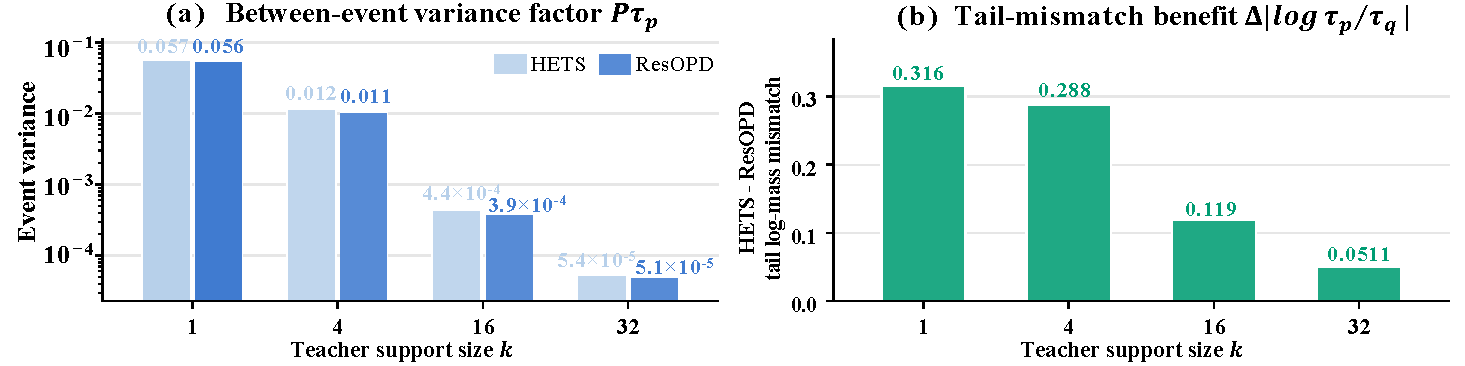
\includegraphics[width=0.9\textwidth]{figs/topk_ablation_v10.pdf}
\caption{在线诊断指标在教师模型 Top-$k$ 支持大小上的表现。
\textbf{(a)} HETS 和 ResOPD 的事件间方差因子 $P\tau_p$，表征头部与尾部划分的缩放系数。
\textbf{(b)} 尾部对数质量不匹配的减少量 ($\text{HETS} - \text{ResOPD}$，通过 $\Delta|\log(\tau_p / \tau_q)|$ 测量)。}
\label{fig:topk-ablation}
\vspace{-4mm}
\end{figure}

附录~\ref{app:fixed-prefix-sweep} 在固定前缀的情况下，研究了支持集大小 $k$ 的影响，报告了确切的协方差迹和NSR。相比之下，此处我们提供了对OPD的端到端在线消融分析。具体而言，表~\ref{tab:topk-breakdown} 和图~\ref{fig:topk-ablation} 展示了在不同教师支持集大小 $k \in \{1, 4, 16, 32\}$ 下的结果。  
如表~\ref{tab:topk-breakdown} 所示，ResOPD 在所有测试的支持集大小下，平均下游准确率均优于HETS，提升幅度从 $+0.11$ 个百分点（在 $k=1$ 处）到 $+1.56$ 个百分点（在 $k=32$ 处）不等。  
然而，尽管下游任务得分始终青睐ResOPD，但ResOPD所提供的内在方差减小优势预计会随着 $k$ 增大而减弱，因为更大的教师支持集自然能捕捉更多的概率质量，从而使得尾部修正的发生频率降低。

图~\ref{fig:topk-ablation} 验证了该机制在表~\ref{tab:topk-breakdown} 所示运行结果中的有效性。在图~\ref{fig:topk-ablation}(a) 中，HETS 和 ResOPD 的方差因子 $P\tau_p$ 几乎相同，均从 $k=1$ 降至 $32$ 以下三个数量级。这直接反映了理论上的 ResOPD--HETS 方差对比与尾部-均值近似质量之间的比例关系。同时，图~\ref{fig:topk-ablation}(b) 显示，ResOPD 在所有支持范围内始终降低了尾部对数质量不匹配度，尤其在紧支持区域的差异最为显著。

\subsection{Rollout采样：默认过滤器与完整支持}
\label{sec:rollout-ablation}
尽管在我们的确切枚举审计（第~\ref{sec:exact-audit} 节）和跨领域迁移实验（第~\ref{sec:cross-domain} 节）中严格遵守了理想化的原始采样条件 $A\sim p_\theta$，我们仍为完整性验证了主要数学结果不依赖于轨迹截断。具体而言，在保持所有其他训练超参数不变的情况下，我们在全支持采样 ($\text{top-}p=1.0$ , $\text{top-}k=-1$ ) 下评估了首个训练轮次。

如表~\ref{tab:full-support-first-epoch} 所示，移除轨迹过滤器后，所有三种评估方法的 AUC 均下降。然而，ResOPD 在基准准确率和轨迹 AUC 两个方面始终优于 HETS 和朴素基准。此外，我们观察到移除轨迹过滤器会导致更长的推理轨迹，并在训练过程中更高频率地触及响应 token 限制。


\subsection{学习率敏感性}
\label{sec:lr-sensitivity}

\begin{table}[t]
\centering
\small
\caption{\textbf{默认滚动与全支持滚动下的首轮次数学性能。}
基准得分和平均值表示第64步的准确率（\%）；$\text{AUC}$ （\%）衡量步骤 $\{0, 6, 32, 64\}$ 内规范化学习曲线面积；  
\textit{默认}：前-$p=0.95$ ，前-$k=20$ ；\textit{全支持}：前-$p=1.0$ ，前-$k=-1$ 。}
\vspace{-2mm}
\label{tab:full-support-first-epoch}
\setlength{\tabcolsep}{5pt}
\renewcommand{\arraystretch}{1.15}
\begin{tabular}{llcccccc}
\toprule
\textbf{Rollout} & \textbf{Method} & \textbf{DeepMath} & \textbf{AIME26} & \textbf{HMMT26} & \textbf{OlymMATH} & \textbf{Avg.} & \textbf{AUC} \\
\midrule
\multirow{3}{*}{Default}
& Naive Top-$k$ rKL & 53.17 & 56.04 & 35.42 & 35.00 & 44.91 & 45.45 \\
& HETS              & 53.17 & 59.17 & 36.93 & 34.50 & 45.94 & 46.12 \\
& ResOPD            & \textbf{54.76} & \textbf{60.00} & \textbf{37.88} & \textbf{35.75} & \textbf{47.10} & \textbf{47.57} \\
\midrule
\multirow{3}{*}{Full}
& Naive Top-$k$ rKL & 45.44 & 55.42 & 35.80 & 34.25 & 42.72 & 44.96 \\
& HETS              & 49.80 & 57.50 & \textbf{37.88} & 35.50 & 45.17 & 45.68 \\
& ResOPD            & \textbf{57.14} & \textbf{60.42} & \textbf{37.88} & \textbf{36.00} & \textbf{47.86} & \textbf{46.79} \\
\bottomrule
\end{tabular}
\end{table}

\paragraph{实验设置与评估协议。}
为了评估在激进步长下的最优化鲁棒性，我们进行了一次受控的学习率扫描（$k=4$），其设置与主数学实验一致，不同之处在于训练被压缩至1~轮次（64次优化器步骤）。所有实验均采用批量大小为16、32K响应预算，并与主实验保持相同的采样配置。在步骤0、6、32和64处的检查点均按照宏-4协议进行评估（对AIME26和HMMT26平均采样16个响应，对DeepMath保留集和OlymMATH采样2个响应）。
\vspace{-4mm}

\begin{table}[t]
\centering
\small
\caption{\textbf{HETS 与 ResOPD 的学习率敏感性。} $\Delta$ 表示 ResOPD 相对于 HETS 的提升。}
\vspace{-2mm}
\label{tab:lr-sensitivity}
\renewcommand{\arraystretch}{1.18}
\setlength{\tabcolsep}{7pt}
\begin{tabular}{@{}l cc c cc c@{}}
\toprule
\multirow{2}{*}{\textbf{Learning Rate}}
& \multicolumn{3}{c}{\textbf{Final Score (\%)}}
& \multicolumn{3}{c}{\textbf{Trajectory AUC (\%)}} \\
\cmidrule(lr){2-4} \cmidrule(l){5-7}
& HETS & ResOPD & $\Delta$
& HETS & ResOPD & $\Delta$ \\
\midrule
$1\times10^{-6}$ & 45.94 & \textbf{47.10} & $+1.16$ & 46.12 & \textbf{47.57} & $+1.45$ \\
$2\times10^{-6}$ & 45.94 & \textbf{46.61} & $+0.67$ & 45.69 & \textbf{46.17} & $+0.48$ \\
$5\times10^{-6}$ & 42.54 & \textbf{46.35} & \textbf{+3.81} & 43.88 & \textbf{47.77} & \textbf{+3.89} \\
\bottomrule
\end{tabular}
\vspace{-4mm}
\end{table}

\paragraph{不同学习率下的性能鲁棒性。}
如表~\ref{tab:lr-sensitivity} 所示，ResOPD 在较高的学习率下表现出显著更强的鲁棒性。当学习率缩放到 $5\times10^{-6}$ 时，HETS 出现严重退化，其最终得分从 $45.94\%$ 降至 $42.54\%$  ($-3.40\%$ )，轨迹 AUC 下降了 $2.24\%$ 。相比之下，ResOPD 保持了稳定的性能（最终得分为 $46.35\%$ ，AUC 为 $47.77\%$ ），其在最终得分上对 HETS 的领先优势扩大至 $+3.81\%$ ，在 AUC 上则扩大至 $+3.89\%$ 。

在该激进学习率下的子基准分解分析显示，ResOPD 在第 64 步的所有四个组成基准上均持续保持正向优势：在 AIME26 上为 $+3.96\%$ ，在 HMMT26 上为 $+2.08\%$ ，在 DeepMath 留出集上为 $+6.94\%$ ，在 OlymMATH 上为 $+2.25\%$ 。我们在附录~\ref{app:lr-sensitivity} 中提供了不同学习率下的详细训练动态。  
\vspace{-4mm}

\paragraph{稳定性边界与失稳模式。}
当学习率进一步缩放至 $1\times10^{-5}$ 时，两种方法均迅速发散，触发严重的梯度裁剪（HETS 为 $4/6$ 步，ResOPD 为 $5/6$ 步），并在六步优化器迭代内出现严重的响应长度坍塌。尽管 ResOPD 在我们默认的训练方案下并未改变最终的发散边界 ($1\times10^{-5}$)，但其粗粒度残差化结构在中等激进的训练环境下提供了显著更宽的稳定性裕度。超出此阈值后，可能需要将更高的学习率与互补的稳定化技术（如更大的批量大小或更紧的裁剪阈值）协同使用，这留待未来工作研究。
\vspace{-4mm}

\subsection{比较双控制终点}
\label{sec:control-comparison}

第\ref{sec:unified} 节中的分析指出，通过 $\gamma$ 可以显著降低尾部内部方差。我们使用 SC-TA ($\gamma=1$ ) 和 ResOPD ($\gamma=0$ ) 对该预测进行了评估，同时保持可观测的粗粒度控制 $\bm B=\bmean_B$ 不变。

\subsubsection{跨分布固定前缀审计}
尽管双控制框架表明，SC-TA ($\gamma=1$ ) 可以缓解 ResOPD ($\gamma=0$ ) 无法处理的尾部波动，但公式~(\ref{eq:event-improvement}) 暗示这种排序依赖于分布，并非普遍成立。为评估跨领域的稳定性，我们在三个自然提示分布（DeepMath \citep{deepmath}、MegaScience \citep{fan2025megascience} 和 SynLogic \citep{liu2026synlogic}）上固定 Qwen3.5-4B/27B 对（前4名支持，64-token 视野），对128条轨迹（8,192个前缀）进行评估，使用20,000次自举重采样。我们追踪规范化的迹方差减小：
\begin{equation}
  \Delta \coloneqq \frac{\mathcal{V}_{\mathrm{SC}} - \mathcal{V}_{\mathrm{ResOPD}}}{\mathcal{V}_{\mathrm{sampled}}},
\end{equation}
负值有利于SC-TA。

如表~\ref{tab:scta-cross-distribution} 所示，总体迹方差在所有三个评估领域中均一致地支持 SC-TA 胜过 ResOPD ($\Delta \in [-0.207, -0.126]$)。同时，前缀级别的交叉现象依然显著（在 SynLogic 中多达 $18.0\%$ 的前缀更倾向于 ResOPD）。这一实证结果验证了我们双控制公式的合理预测：尽管设定 $\gamma=1$ 可能在期望上带来更低的方差，但局部方差排序仍严格依赖于前缀，而非全局统一。

原则上，可以从前训练分布中预先选择一组提示，以经验方式校准最优系数 $\gamma^\star$，从而在最优化过程中可能实现额外的方差减小（尽管 $\gamma^\star$ 会随着模型权重自然演化）。然而，在实践中，我们的实验表明，与固定启发式方法 $\gamma=1$ 相比，这种校准带来的增量收益微乎其微。因此，为保持简洁，我们省略进一步讨论。

\begin{table}[t]
\caption{\textbf{SC-TA 与 ResOPD 在自然提示分布下的协方差迹排序对比。}}
\vspace{-2mm}
\label{tab:scta-cross-distribution}
\centering
\small
\setlength{\tabcolsep}{6.0pt}
\begin{tabular}{@{}lccc@{}}
\toprule
Dataset & $\mathcal{V}_{\mathrm{SC}} / \mathcal{V}_{\mathrm{ResOPD}}$ & $\Delta$ & ResOPD-Lower Prefixes \\
\midrule
DeepMath    & 0.512 & $-0.126$ & \phantom{0}6.8\% \\
MegaScience & 0.532 & $-0.207$ & 11.3\% \\
SynLogic    & 0.558 & $-0.161$ & 18.0\% \\
\bottomrule
\end{tabular}
\vspace{-2mm}
\end{table}

\begin{table}[t]
\caption{\textbf{训练更新过程中的匹配评估曲线（\%）。}
在 Qwen3.5-27B-to-4B 蒸馏上评估，涵盖 AIME26/HMMT26（平均@16）和保留的 DeepMath/OlymMATH（平均@2）。}
\vspace{-2mm}
\label{tab:scta-curve}
\centering
\small
\setlength{\tabcolsep}{5.5pt}
\begin{tabular}{@{}lcccccc@{}}
\toprule
Method & Base (Step 0) & Step 6 & Step 32 & Step 64 & Step 128 & Step 192 \\
\midrule
HETS  & 42.85 & \textbf{48.86} & 45.04 & 45.94 & 46.60 & 45.72 \\
ResOPD   & 42.85 & 48.23 & \textbf{47.95} & 47.10 & 47.71 & \textbf{50.12} \\
SC-TA & 42.85 & 47.66 & 46.69 & \textbf{47.26} & \textbf{48.27} & 46.33 \\
\bottomrule
\end{tabular}
\vspace{-4mm}
\end{table}

\subsubsection{下游评估对比}
虽然SC-TA将固定前缀残差协方差迹减半，但这一优势并不一定转化为下游准确率的提升。如表~\ref{tab:scta-curve}所示，SC-TA并未在下游任务中表现出对ResOPD的一致优势：在多个中间检查点上表现略强，而ResOPD在最终得分上更高，轨迹级AUC保持相近。

This decoupling between gradient covariance trace and downstream performance is informative rather than contradictory. While lower estimator variance validates the two-control residualization mechanism locally, downstream benchmark accuracy reflects the global trajectory of policy updates.
Consequently, while SC-TA exhibits lower overall variance across the evaluated audit sets, ResOPD retains strong aggregate performance in this evaluated setting without explicitly subtracting the additional within-tail score fluctuation.
\vspace{-4mm}

\FloatBarrier
\section{结论}

我们提出了ResOPD，这是一种在稀疏教师反馈下针对全词表反向KL蒸馏的合理估计量。通过解析地整合可观察到的粗粒度分布，并仅对未解决的细尾残差进行采样，ResOPD在评估情景中降低了方差，同时在祖先同策略采样下保持了确切的无偏性，且无需增加教师负载或额外前向传播。基于理论分析、精确协方差审计以及在数学、科学和编程任务上的实证评估，ResOPD在评估情景中表现出更高的综合下游得分。


\FloatBarrier

\Needspace{5\baselineskip}
\renewcommand{\bibfont}{\small}
\setlength{\bibsep}{3pt plus 1pt minus 1pt}
\bibliographystyle{plainnat}
\bibliography{refs}

\clearpage
\appendix
\section{详细的估计量推导}
\label{app:theory}

正文给出了估计量、其无偏性恒等式以及统一的方差分析。附录提供了详细的 Top-$k$ 偏差推导和单控制预言机计算，包括完整粗粒度分布的边界项抵消。

\subsection{三种有偏的 Teacher \texorpdfstring{Top-$k$}{Top-k} 反向 KL}
\label{app:topk-bias}

本小节区分了三种常被混淆的操作：
在头部对两个分布进行重归一化、截断标量反KL目标，以及仅截断停止系数的梯度。每种操作均可从教师模型的 Top-$k$ 中计算得出，但它们均无法准确估计完整词表反KL目标的梯度。此处的“偏差”是相对于该目标梯度而言的，而非蒙特卡罗采样偏差。固定支持集 $S$ 与教师概率，
令 $z$ 为无限制的学生Logit，定义
\begin{equation}
 \begin{gathered}
 R\coloneqq\sum_i p_i r_i=\KL(p\|q),\qquad
 R_S\coloneqq\sum_{i\in S}p_i r_i,\\
 P\coloneqq\sum_{i\in S}p_i,\qquad
 Q\coloneqq\sum_{i\in S}q_i.
 \end{gathered}
\end{equation}
确切的完整rKL Logit梯度，作为以下参考：
\begin{equation}
 [\nabla_z R]_j=p_j(r_j-R).
 \label{eq:full-rkl-logit-gradient}
\end{equation}

\paragraph{重规范化Top-$k$ 反向KL。}
定义 $\widetilde p_i=p_i/P$ 、$\widetilde q_i=q_i/Q$ 和 $\widetilde r_i=\log(\widetilde p_i/\widetilde q_i)$ 为 $i\in S$，其中包含 $\widetilde R=\sum_{i\in S}\widetilde p_i\widetilde r_i$。由于 $\widetilde p_i=\exp (z_i)/\sum_{\ell\in S}\exp (z_\ell)$，目标函数及其 Logit 梯度为
\begin{equation}
 \begin{aligned}
 L_{\mathrm{renormalized}}
 &=\sum_{i\in S}\widetilde p_i
   \log\frac{\widetilde p_i}{\widetilde q_i},\\
 [\nabla_z L_{\mathrm{renormalized}}]_j
 &=\ind\{j\in S\}\widetilde p_j
   (\widetilde r_j-\widetilde R).
 \end{aligned}
 \label{eq:renorm-topk-gradient}
\end{equation}
每个尾部Logit分量恰好为零，而  
公式~(\ref{eq:full-rkl-logit-gradient}) 在此处通常不为零。全局最小值是集合
\begin{equation}
 \widetilde p_i=\widetilde q_i
 \quad(i\in S)
 \quad\Longleftrightarrow\quad
 p_i=\frac{P}{Q}q_i\quad(i\in S),
 \label{eq:renorm-topk-optimum}
\end{equation}
具有任意的 $P$  和任意的尾部形状。因此，重规范化仅学习条件头部分布；它既无法确定头部质量，也无法识别被省略的条件分布。

\paragraph{标量截断的Top-$k$ 反向KL。}
未规范化的标量捷径为
$L_{\mathrm{truncated}}=R_S=\sum_{i\in S}p_i r_i$ 。写作
$C_S\coloneqq\sum_{i\in S}p_i(r_i+1)=R_S+P$ ，直接微分可得
\begin{equation}
 \begin{aligned}
 \nabla_\theta L_{\mathrm{truncated}}
 &=\bhead+\nabla_\theta P,\\
 [\nabla_z L_{\mathrm{truncated}}]_j
 &=\ind\{j\in S\}p_j(r_j+1)-p_jC_S.
 \end{aligned}
 \label{eq:scalar-truncated-gradient}
\end{equation}
因此，其相对于完整rKL的偏差为
$\nabla_\theta P-\tau_p\bmean_{\mathrm{tail}}$ 。特别是，当
$j\notin S$ ，$[\nabla_z L_{\mathrm{tr}}]_j=-p_jC_S$ ；当 $C_S>0$ 时，
梯度下降会增加每一个被省略的Logit。

相应的全局最优解使失效更加明显。对于每个头坐标，
\begin{equation}
 x\log\frac{x}{q_i}\geq-\frac{q_i}{e},
 \qquad\text{with equality iff }x=\frac{q_i}{e}.
\end{equation}
由于 $\sum_{i\in S}q_i/e=Q/e<1$，所有坐标极小值联合可行，因此
\begin{equation}
 p_i^\star=\frac{q_i}{e}\quad(i\in S),\qquad
 P^\star=\frac{Q}{e},\qquad
 \sum_{j\notin S}p_j^\star=1-\frac{Q}{e},
 \label{eq:scalar-truncated-optimum}
\end{equation}
在尾部内部具有任意分配。即使 $Q$  接近一，此目标也更倾向于在教师头部之外保留大约 $1-1/e$  的学生质量；因此，尾部推动是一种目标层面的特性，而不仅仅是瞬时梯度符号。

\paragraph{停止系数的Top-$k$ 反向KL梯度。}
停止对系数的调整会消除 $\nabla P$ 边界项，但会使尾部期望保持未校正状态：
\begin{equation}
  \begin{gathered}
    \bgrad_{\text{Top-}k} \coloneqq \sum_{i \in S} \operatorname{stopgrad}(p_i r_i) \bscore_i = \bhead, \\
    [\bgrad_{\text{Top-}k}]_j = \ind\{j \in S\} p_j r_j - p_j R_S, \qquad
    \bgrad_{\text{Top-}k} - \bgrad = -\tau_p \bmean_{\mathrm{tail}}.
  \end{gathered}
  \label{eq:stopped-topk-gradient-bias}
\end{equation}
在无限制的类别Logit空间中，若尾部非空，则梯度消失（$\bgrad_{\text{Top-}k} = \mathbf{0}$）迫使 $R_S = 0$ 通过尾部组件（$j \notin S$），这随后意味着对所有头部组件（$i \in S$）有 $r_i = 0$。因此，$p_i = q_i$ 在头部成立，正确匹配了整体尾部质量（$1 - P = 1 - Q$）；然而，尾部上的条件分布仍不受约束且任意。尽管这种停梯度公式在三种启发式方法中对潜在目标的影响最小，但只要尾部向量非零，它仍具有内在的有偏性。HETS 和 ResOPD 通过引入采样尾部修正来恢复缺失的期望，从而解决这一残余偏差。

\subsection{单控制残差化及其方差最优}
\label{app:single-control}

使用公式~(\ref{eq:head-tail-definitions}) 的头/尾记号，令
$J=\ind\{A\notin S\}$ ，并令 $\bm B$ 为任意在采样 $A\sim p$ 之前停止的有限前缀可测向量。考虑单控制估计量
\begin{equation}
 \widehat{\bgrad}(\bm B)
 \coloneqq
 \bhead+\tau_p\bm B+J(\btoken_A-\bm B).
 \label{eq:single-control-estimator}
\end{equation}
它对每一个这样的 $\bm B$ 都是无偏的：
\begin{equation}
 \E[\widehat{\bgrad}(\bm B)]
 =\bhead+\tau_p\bm B
  +\tau_p(\bmean_{\mathrm{tail}}-\bm B)
 =\bgrad.
 \label{eq:single-control-unbiased}
\end{equation}
在给定 $J=0$ 的条件下，其值为确定性向量
$\bhead+\tau_p\bm B$ 。在给定 $J=1$ 的条件下，其均值为
$\bhead+\tau_p\bm B+\bmean_{\mathrm{tail}}-\bm B$ ，协方差为
$\Cov_{\mathrm{tail}}(\btoken_A)$ 。两个条件均值之差为
$\bmean_{\mathrm{tail}}-\bm B$ 。因此，全协方差定律给出
\begin{equation}
 \mathcal V(\widehat{\bgrad}(\bm B))
 =\tau_p\mathcal V_{\mathrm{tail}}(\btoken_A)
 +P\tau_p\lVert\bmean_{\mathrm{tail}}-\bm B\rVert_2^2.
 \label{eq:single-control-variance}
\end{equation}
第一项与 $\bm B$ 无关。因此，每当
$0<P<1$ 时，唯一的迹-协方差最小化器及其确切遗憾为
\begin{equation}
 \begin{aligned}
 \bm B^\star&=\bmean_{\mathrm{tail}},\\
 \mathcal V(\widehat{\bgrad}(\bm B))
 -\mathcal V(\widehat{\bgrad}(\bmean_{\mathrm{tail}}))
 &=P\tau_p\lVert\bm B-\bmean_{\mathrm{tail}}\rVert_2^2.
 \end{aligned}
 \label{eq:single-control-oracle}
\end{equation}
该预言机消除了所有头对尾事件的方差，但在稀疏教师接口下不可用，因为它需要完整的条件尾部均值。

HETS和ResOPD是两种载荷兼容的选择
\begin{equation}
 \widehat{\bgrad}^{\mathrm{HETS}}=\widehat{\bgrad}(\bm 0),
 \qquad
 \widehat{\bgrad}^{\mathrm{ResOPD}}=\widehat{\bgrad}(\bmean_B).
\end{equation}
它们相对于单控制预言机的遗憾分别是
$P\tau_p\lVert\bmean_{\mathrm{tail}}\rVert_2^2$  和
$P\tau_p\lVert\bmean_{\mathrm{tail}}-\bmean_B\rVert_2^2$ 。相减得
\begin{equation}
  \mathcal{V}(\widehat{\bgrad}^{\mathrm{HETS}}) - \mathcal{V}(\widehat{\bgrad}^{\mathrm{ResOPD}}) = P\tau_p \!\left( 2\langle\bmean_{\mathrm{tail}}, \bmean_B\rangle - \lVert\bmean_B\rVert_2^2 \right).
  \label{eq:hets-cfr-variance-appendix}
\end{equation}
因此，确切地当 $\bmean_B$ 比 HETS 对照 $\bm 0$ 更接近 $\bmean_{\mathrm{tail}}$ 时，ResOPD 具有更低的迹协方差；不断言无条件排序。

仍需验证为何在没有精细教师尾部的情况下 $\bmean_B$ 仍然可用。对 $k$  head token 和一个 tail 桶的完整粗粒度分布的反向 KL 为
\begin{equation}
 L_{\mathrm{coarse}}
 \coloneqq
 \sum_{i\in S}p_i\log\frac{p_i}{q_i}
 +\tau_p\log\frac{\tau_p}{\tau_q}.
\end{equation}
由于
$\nabla\tau_p=\tau_p\bar{\bscore}_{\mathrm{tail}}=-\nabla P$ ,
直接微分
可得
\begin{equation}
 \begin{aligned}
 \nabla L_{\mathrm{coarse}}
 &=\bhead+\nabla P+(b+1)\nabla\tau_p\\
 &=\bhead+b\nabla\tau_p
  =\bhead+\tau_p\bmean_B
  =\bgrad_{\mathrm{coarse}}.
 \end{aligned}
\end{equation}
边界项相互抵消，因为尾部伪token完成了粗粒度支持。这就是为什么 $\bgrad_{\mathrm{coarse}}$ 是一个确切的梯度（但有偏），即使 $\bmean_B$ 未必等于真实的条件细粒度尾部均值。

\FloatBarrier
\section{详细的训练和评估配置}
\label{app:hyperparameters}


表格。~\ref{tab:opd-hyperparameters} 和 ~\ref{tab:qwen3-opd-hyperparameters} 收集了主数学领域和跨领域运行的完整情景设置。它们的采样假设在第~\ref{subsec:evidence} 和 ~\ref{sec:ex-setup} 节中进行了讨论；匹配的全支撑数学消融结果在第~\ref{sec:rollout-ablation} 节中报告。

\begin{table}[t]
\caption{\textbf{主数学OPD实验配置和超参数。}}
\label{tab:opd-hyperparameters}
\centering
\small
\renewcommand{\arraystretch}{1.18}
\setlength{\tabcolsep}{6pt}
\begin{tabular}{@{}lll@{}}
\toprule
\textbf{Category} & \textbf{Hyperparameter} & \textbf{Configuration / Value} \\
\midrule

\multirow{2}{*}{\textbf{Models}}
& Student model & Qwen3.5-4B \\
& Teacher model & Qwen3.5-27B \\
\midrule

\multirow{2}{*}{\textbf{Data}}
& Training dataset & 1{,}024 prompts sampled from DeepMath-103K \\
& Max prompt length & 2{,}048 \\
\midrule

\multirow{5}{*}{\textbf{Sampling}}
& Enable thinking & True \\
& Max response length & 32{,}768 (training and evaluation) \\
& temperature & 1.0 \\
& top-$p$ & 0.95 \\
& top-$k$ & 20 \\
\midrule

\multirow{5}{*}{\textbf{Training}}
& Training epochs & 3 \\
& Global batch size & 16 \\
& Optimizer & AdamW \\
& Gradient clipping & 1.0 \\
& Learning rate & $1\times10^{-6}$ \\
\midrule

\multirow{4}{*}{\textbf{System \& Hardware}}
& Compute infrastructure & $16\times$ NVIDIA H200 GPUs \\
& Resource allocation & 8 GPUs for Student rollout, 4 for Student training, \\
& & 4 for hosting the Teacher inference service \\
& Software frameworks & Training: verl \quad Inference: vLLM \\
\bottomrule
\end{tabular}
\end{table}


\section{逐步评估结果}

\subsection{数学运算能力发展实验}
\label{app:math-learning-trajectories}

\begin{table}[t]
\caption{\textbf{跨领域Qwen3 OPD实验配置与超参数。}}
\label{tab:qwen3-opd-hyperparameters}
\centering
\small
\renewcommand{\arraystretch}{1.18}
\setlength{\tabcolsep}{6pt}
\begin{tabular}{@{}lll@{}}
\toprule
\textbf{Category} & \textbf{Hyperparameter} & \textbf{Configuration / Value} \\
\midrule
\multirow{2}{*}{\textbf{Models}}
& Student model & Qwen3-4B \\
& Teacher model & Qwen3-30B-A3B-Instruct-2507 \\
\midrule
\multirow{3}{*}{\textbf{Data}}
& Training dataset & 30,000 deduplicated prompts; \\
& & Math/Code/Science: 10,000 each \\
& Max prompt length & 1,024 \\
\midrule
\multirow{5}{*}{\textbf{Sampling}}
& Enable thinking & False \\
& Max response length & 8192 (training) and 32768 (evaluation) \\
& temperature & 1.0 \\
& top-$p$ & 1.0 \\
& top-$k$ & $-1$ \\
\midrule
\multirow{7}{*}{\textbf{Training}}
& Training steps & 100 \\
& Global batch size & 288 \\
& Optimizer & AdamW \\
& Gradient clipping & 1.0 \\
& Peak learning rate & $5\times10^{-6}$ \\
& LR schedule & 10-step warmup; \\
& & cosine decay to $0.1\times$ peak \\
\midrule
\multirow{4}{*}{\textbf{System \& Hardware}}
& Compute infrastructure & $16\times$ NVIDIA H200 GPUs \\
& Resource allocation & 8 GPUs for student rollout, 4 for student training, \\
& & 4 for hosting the teacher inference service \\
& Software frameworks & Training: verl \quad Inference: vLLM \\
\bottomrule
\end{tabular}
\end{table}


图~\ref{fig:estimator-learning} 展示了在评估套件上的训练轨迹。  
在 DeepMath 的保留集上，ResOPD 显现出稳定的后期增益，在所有估计量中达到了最高的最终准确率。  
尽管像 TA-OPD 和 Teacher Top-$k$  vOPD 这样的竞争性基准表现出持续改进，但在最终检查点处仍不及 ResOPD。与此同时，Sampled-token OPD 在早期达到峰值后严重恶化，而 HETS 则在后期出现下降。  
在外部数学竞赛中也呈现出类似趋势：尽管 TA-OPD 保持了强劲的中期轨迹表现，vOPD 也保持竞争力，但 ResOPD 展现出更优的后期韧性，并在最后一步彻底超越所有其他方法，避免了如 Sampled-token OPD 和 HETS 等估计量所观察到的峰值后退化现象。

结合论文中其他部分报告的固定前缀协方差迹降低和改进的在线训练诊断，这些轨迹与所提出的粗尾残差化方法减少随机梯度噪声并提升后期最优化稳定性一致。

\subsection{跨领域OPD实验}
\label{app:cross-qwen3}

\begin{figure}[t]
\centering
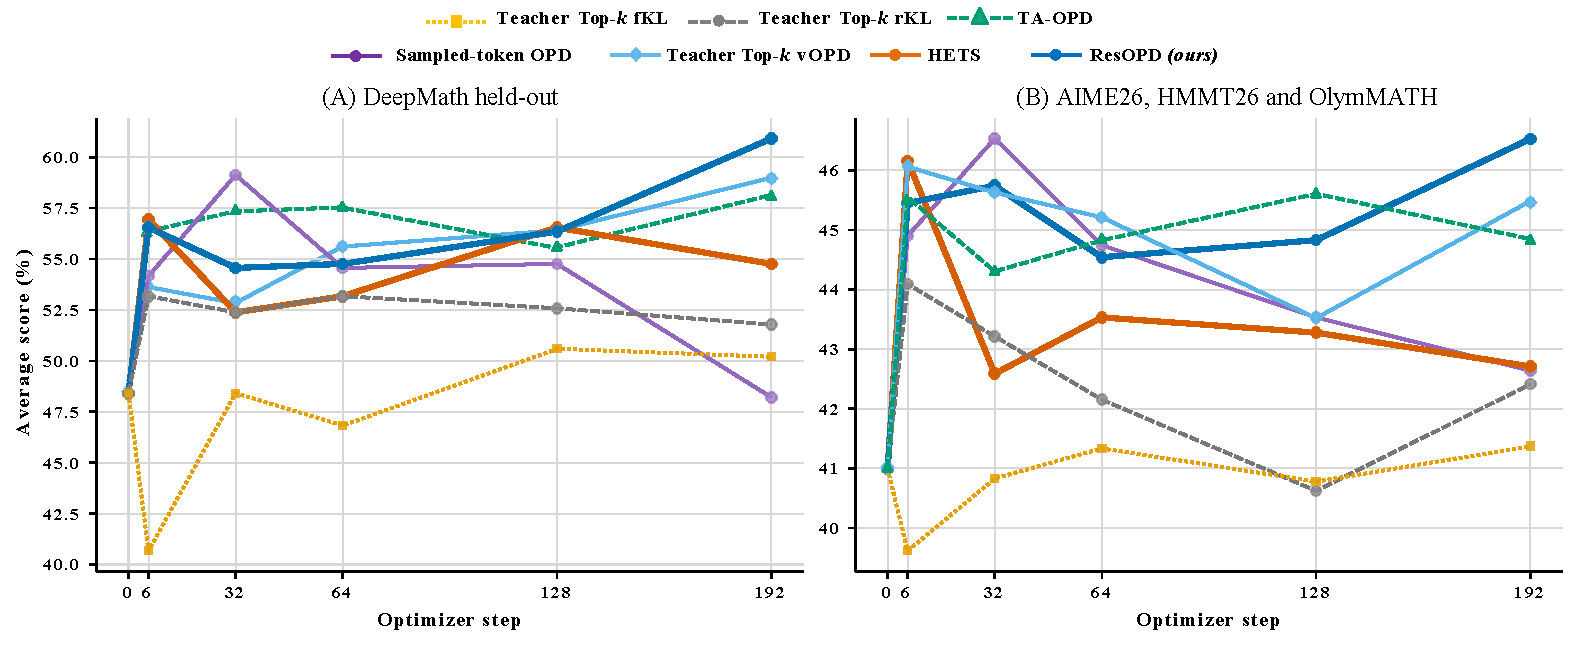
\includegraphics[width=0.85\textwidth]{figs/math_step_v4.pdf}
\caption{\textbf{分步学习曲线} 对应于表~\ref{tab:math-terminal} 在 DeepMath 留出集（左）和外部竞赛（右）上的结果，覆盖 192 个优化器步骤。}
\label{fig:estimator-learning}
\end{figure}

图~\ref{fig:qwen3-transfer-curves} 展示了在所有四个基准上的固定训练进度（步骤 0、10、25、50 和 100）下，检查点评估轨迹。在代码基准（LiveCodeBench v5 和 v6）上，ResOPD 和 HETS 快速收敛，并在整个训练过程中显著优于采样 token 的 OPD，其中 ResOPD 达到了最高的整体轨迹 AUC。相比之下，科学基准表现出混合的领域动态：在 GPQA-D 上，采样 token 的 OPD 展现了更优的保留能力和最终准确率；而 ResOPD 在整个训练步骤中保持竞争力，并在 SuperGPQA 上取得了最佳终端性能。这些轨迹证实，尽管采样 token 的 OPD 在专业科学推理任务中表现强劲，但 ResOPD 在代码任务上提供了良好的迁移性能，同时不牺牲整体多领域平衡性。

\begin{figure}[htbp]
  \centering
  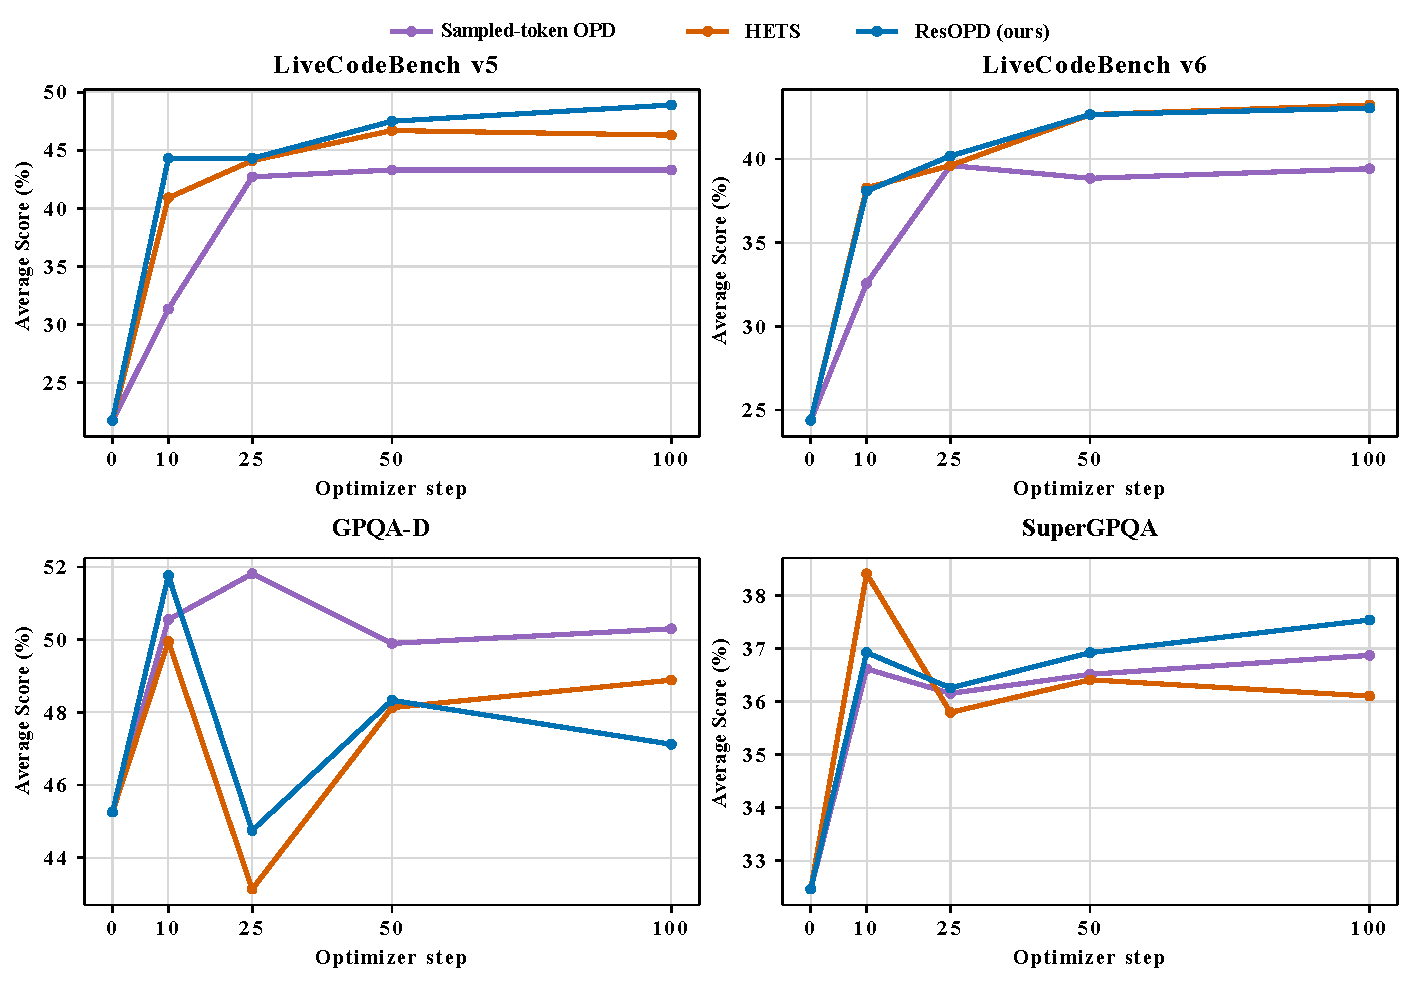
\includegraphics[width=0.85\columnwidth]{figs/qwen3_4b30_transfer_curves_v2.pdf}
    \caption{\textbf{从 Qwen3-30B-A3B-Instruct 到 Qwen3-4B 的跨领域蒸馏过程中的评估轨迹}，在优化器步骤（0、10、25、50 和 100）处。}
    \label{fig:qwen3-transfer-curves}
\end{figure}

\FloatBarrier
\section{诊断详情}
\label{app:math-curves}

\subsection{在线残余力矩测量}
\label{app:online-residual-moments}

在优化器更新 $u$ 时，令 $i \in \{1, \dots, B_u\}$  索引非空采样响应，$t \in \{1, \dots, T_{ui}\}$  索引其有效 token。我们定义标量支持残差及其组成部分为
\begin{equation}
  P_{uit} \coloneqq p_\theta(S_{uit} \mid x_{uit}), \qquad
  H_{uit} \coloneqq \ind\{A_{uit} \in S_{uit}\}, \qquad
  Z_{uit} \coloneqq H_{uit} - P_{uit}.
  \label{eq:online-support-residual}
\end{equation}
此处，$P_{uit}$ 表示分配给传输的教师模型 \text{Top-}$k$ 支持集 $S_{uit}$ 的学生模型概率质量，而 $H_{uit}$ 表示采样的学生 token 是否落入该集合。在确切的同策略采样下，残差条件期望为零，$\E[Z_{uit} \mid x_{uit}] = 0$ ，其条件方差为 $\E[Z_{uit}^2 \mid x_{uit}] = P_{uit}(1 - P_{uit})$ 。更一般地，其未中心化的二阶矩同时捕捉了内在采样变异性以及任何实现的校准漂移。

图~\ref{fig:training-dynamics-event-g0} 报告了该量的两种诊断聚合。面板~C 展示了掩码 token 级别的二阶矩：
\begin{equation}
  M_{2,\mathrm{tok}}^{(u)} = \frac{1}{\sum_{i=1}^{B_u} T_{ui}} \sum_{i=1}^{B_u} \sum_{t=1}^{T_{ui}} Z_{uit}^2,
  \label{eq:online-token-m2}
\end{equation}
而面板D通过先对每次反应内的数据求平均，再对各反应进行均匀加权，来评估轨迹层面的方差：
\begin{equation}
  \bar{Z}_{ui} = \frac{1}{T_{ui}} \sum_{t=1}^{T_{ui}} Z_{uit}, \qquad
  M_{2,\mathrm{traj}}^{(u)} = \frac{1}{B_u} \sum_{i=1}^{B_u} \bar{Z}_{ui}^2.
  \label{eq:online-trajectory-m2}
\end{equation}
直观上，$M_{2,\mathrm{tok}}$ 捕捉了未解析的头对尾事件的瞬时幅度（这在图~\ref{fig:topk-ablation} 中被用于近似事件间方差因子 $P\tau_p$），而 $M_{2,\mathrm{traj}}$ 则衡量了在序列滚动过程中持续存在的、带有符号的事件不平衡。定义批量均值 $\bar{Z}_u = B_u^{-1} \sum_{i=1}^{B_u} \bar{Z}_{ui}$ ，轨迹均值的经验标准差为
\begin{equation}
  \widehat{\operatorname{SE}}(\bar{Z}_u) = \sqrt{\frac{\max\{M_{2,\mathrm{traj}}^{(u)} - \bar{Z}_u^2, 0\}}{B_u - 1}}.
  \label{eq:online-trajectory-se}
\end{equation}

ResOPD 的连接在标量系数层面上是确切的。注意到尾部指标和尾部质量满足 $J_{uit} = 1 - H_{uit}$ 和 $\tau_{p,uit} = 1 - P_{uit}$ ，我们得到 $Z_{uit} = \tau_{p,uit} - J_{uit}$ 。将其代入式~(\ref{eq:residualization}) 得
\begin{equation}
  \widehat{\bgrad}_{uit}^{\mathrm{ResOPD}} - \widehat{\bgrad}_{uit}^{\mathrm{HETS}} = Z_{uit} \bmean_{B,uit}.
  \label{eq:online-residual-cfr-link}
\end{equation}
因此，这两个 $M_2$  指标直接追踪了随机标量对 ResOPD 桶控制幅度及其序列级持续性的调节。由于它们有意忽略了 $\lVert\bmean_{B,uit}\rVert$ 、其与细尾均值的对齐以及尾部内部的正交波动，因而作为计算轻量、机制对齐的在线诊断工具，而非完整的协方差估计量或固定前缀 NSR 的替代品。最后，尽管 $Z$  可以在稀疏的 Top-$k$  目标中被简单记录，但直接的 Top-$k$  rKL 缺乏采样尾部修正，且相对于真实 rKL 目标始终存在有偏性。因此，其零动作采样方差无法与图 C 和图 D 中无偏的 vOPD、HETS 以及 ResOPD 估计量相比较。


\subsection{有限梯度枚举检查}
\label{app:finite-check}

我们还在无蒙特卡罗误差的情况下，验证了四动作 Softmax 的无偏性恒等式。学生和教师的概率分别为 $(0.35,0.30,0.20,0.15)$ 和 $(0.60,0.25,0.10,0.05)$，前两个动作构成教师的 Top-2 支持集。我们直接对完整的反向 KL 散度进行微分，枚举每个可能的学生动作，并以其确切的学生动作概率加权估计量的梯度。所得的 HETS 期望与稠密全反向 KL 梯度的最大绝对误差为 $5.6\times10^{-17}$ 。

ResOPD 相对于 HETS 将逐动作向量改变了 $(\tau_p-J)\bmean_B$。由于相同的枚举具有 $\E[J]=\tau_p$，该修正的总和恰好为零，ResOPD 恢复了相同的稠密梯度。这种有限检查补充了公式~(\ref{eq:residualization}) 中的符号恒等式：它验证了停止系数和支持掩码的实现语义，但它并不是关于协方差或下游准确率的经验证据。

\subsection{完整的冻结前缀支持诊断}
\label{app:fixed-prefix-sweep}

\begin{table}[t]
\caption{\textbf{在固定教师模型 Top-$k$  输出负载下的支持集大小 ($k$ ) 检查。}
``移除的方差'' 表示相对于采样 token 的 OPD，经验协方差迹的减小量。负载包含 $k$  个 Top-$k$  项以及采样 token（各含 INT32 ID 和 FP32 概率对数）。学生质量与头部命中分别表示落在 Top-$k$  支持集中的预测概率和经验概率。各情景下最佳方差减小和 NSR 以 \textbf{粗体} 标出。}
\label{tab:fixed-prefix-sweep}
\centering
\small
\renewcommand{\arraystretch}{1.16}
\setlength{\tabcolsep}{4.0pt}

\begin{tabular*}{\textwidth}{@{\extracolsep{\fill}}lrrccrrrr@{}}
\toprule
\multirow{2}{*}{\shortstack[l]{Dataset \\ Student/Teacher}}
& \multirow{2}{*}{$k$}
& \multirow{2}{*}{\shortstack{Payload \\ (B/token)}}
& \multirow{2}{*}{\shortstack{Student \\ mass}}
& \multirow{2}{*}{\shortstack{Head \\ Hit}}
& \multicolumn{2}{c}{Var. Removed (\%) $\uparrow$}
& \multicolumn{2}{c}{NSR $\downarrow$} \\
\cmidrule(lr){6-7}\cmidrule(l){8-9}
& & & & & HETS & ResOPD & HETS & ResOPD \\
\midrule
\multirow{4}{*}{\shortstack[l]{\textbf{GSM8K} \\ 0.8B/4B}}
& 1  & 16  & $75.0\%$ & $74.8\%$  & $-0.5$ & $\mathbf{20.5}$ & 5.446 & $\mathbf{4.310}$ \\
& 4  & 40  & $93.1\%$ & $92.9\%$  & 27.3   & $\mathbf{52.5}$ & 3.940 & $\mathbf{2.573}$ \\
& 16 & 136 & $97.7\%$ & $97.9\%$  & 62.6   & $\mathbf{75.3}$ & 2.027 & $\mathbf{1.337}$ \\
& 64 & 520 & $99.3\%$ & $99.7\%$  & 85.1   & $\mathbf{89.5}$ & 0.807 & $\mathbf{0.570}$ \\
\addlinespace[0.25em]
\multirow{3}{*}{\shortstack[l]{\textbf{HMMT26} \\ 4B/27B}}
& 1  & 16  & $89.1\%$ & $89.3\%$   & $-1.0$ & $\mathbf{32.0}$ & 6.656 & $\mathbf{4.479}$ \\
& 4  & 40  & $99.1\%$ & $98.8\%$   & 55.8   & $\mathbf{75.3}$ & 2.914 & $\mathbf{1.630}$ \\
& 16 & 136 & $99.9\%$ & $100.0\%$  & 89.8   & $\mathbf{94.2}$ & 0.675 & $\mathbf{0.382}$ \\
\bottomrule
\end{tabular*}
\end{table}


\begin{figure}[t]
\centering
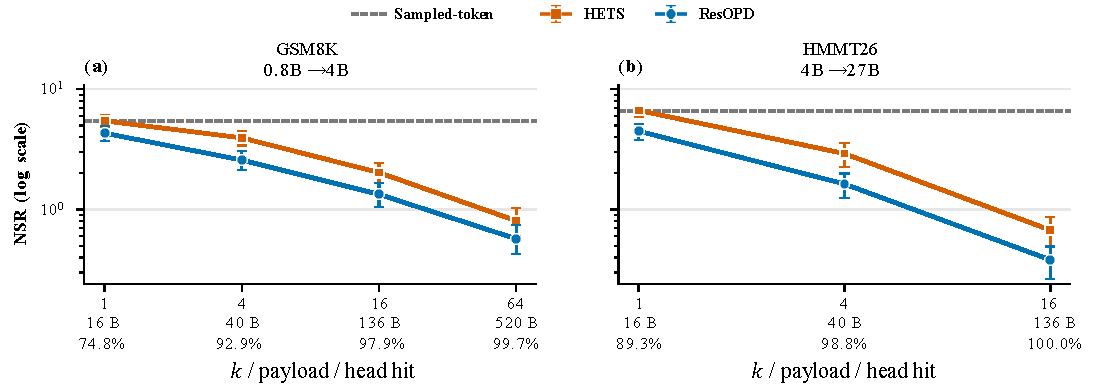
\includegraphics[width=0.96\textwidth]{figs/fixed_prefix_support_strata_v2.pdf}
\caption{\textbf{在基准测试中对冻结前缀支持大小（$k$）的全面诊断。} 
ResOPD 在 GSM8K 和 HMMT 上所有评估的支持大小下，持续降低了无量纲 NSR（对数尺度）。坐标轴标注详细说明了传输的教师端支持大小 $k$、相应的通信负载（字节/token）以及经验头部命中概率。误差条表示 95\% 轨迹级自助法置信区间。}
\label{fig:fixed-prefix-diagnostics}
\end{figure}

在表~\ref{tab:fixed-prefix-sweep} 中的两个测试套件中，ResOPD 在每个匹配的支持大小下均持续优于 HETS，实现了更高的协方差-迹消除和更低的 NSR。将 $k$ 从 $4$ 扩展到 $16$ 和 $64$ 会使传输成本分别增加 $3.4\times$ 和 $13\times$  ($40 \to 136 \to 520$ \,B/token)，但边际方差收益递减。关键的是，头部命中率表明仅高支持覆盖是不够的：即使头部质量达到 $98.8\%$  ($k=4$  on HMMT26)，稀有 $1.2\%$  尾部采样仍导致显著的 HETS--ResOPD 方差差距（$55.8\%$ 与 $75.3\%$  被消除）。此外，在 $k=1$ 处，HETS 表现出负向减少（$-1.0\%$ ），而 ResOPD 稳定地消除了 $32.0\%$  的梯度方差。这有力证实了公式~(\ref{eq:hets-cfr-variance-appendix}) 中的理论条件，确认尽管尾部采样的名义概率质量较低，但未校正的尾部采样仍主导残余梯度噪声。

\subsection{不同学习率下的训练动态}
\label{app:lr-sensitivity}


\paragraph{潜在的训练动态。}
图~\ref{fig:lr-sensitivity} 中的训练轨迹揭示了这种发散背后的两个清晰机制。首先，在梯度幅值方面，ResOPD 在 $5\times10^{-6}$ 时保持显著更低的裁剪前梯度范数（均值 $0.43$  vs.\ $0.48$ ；99\%分位数 $0.97$  vs.\ $1.84$ ），且完全避免了梯度裁剪（$0/64$  步 vs.\ $2/64$  步，对应 HETS）。其次，在残差稳定化方面，图 (B)--(D) 显示，ResOPD 一致地抑制了支持集质量差距 ($Q-P$ )，并压制了 token 级和轨迹级残差二阶矩 ($M_2$ )，这与该步长下观察到的更稳定的学习轨迹一致。

\begin{figure}[t]
  \centering
  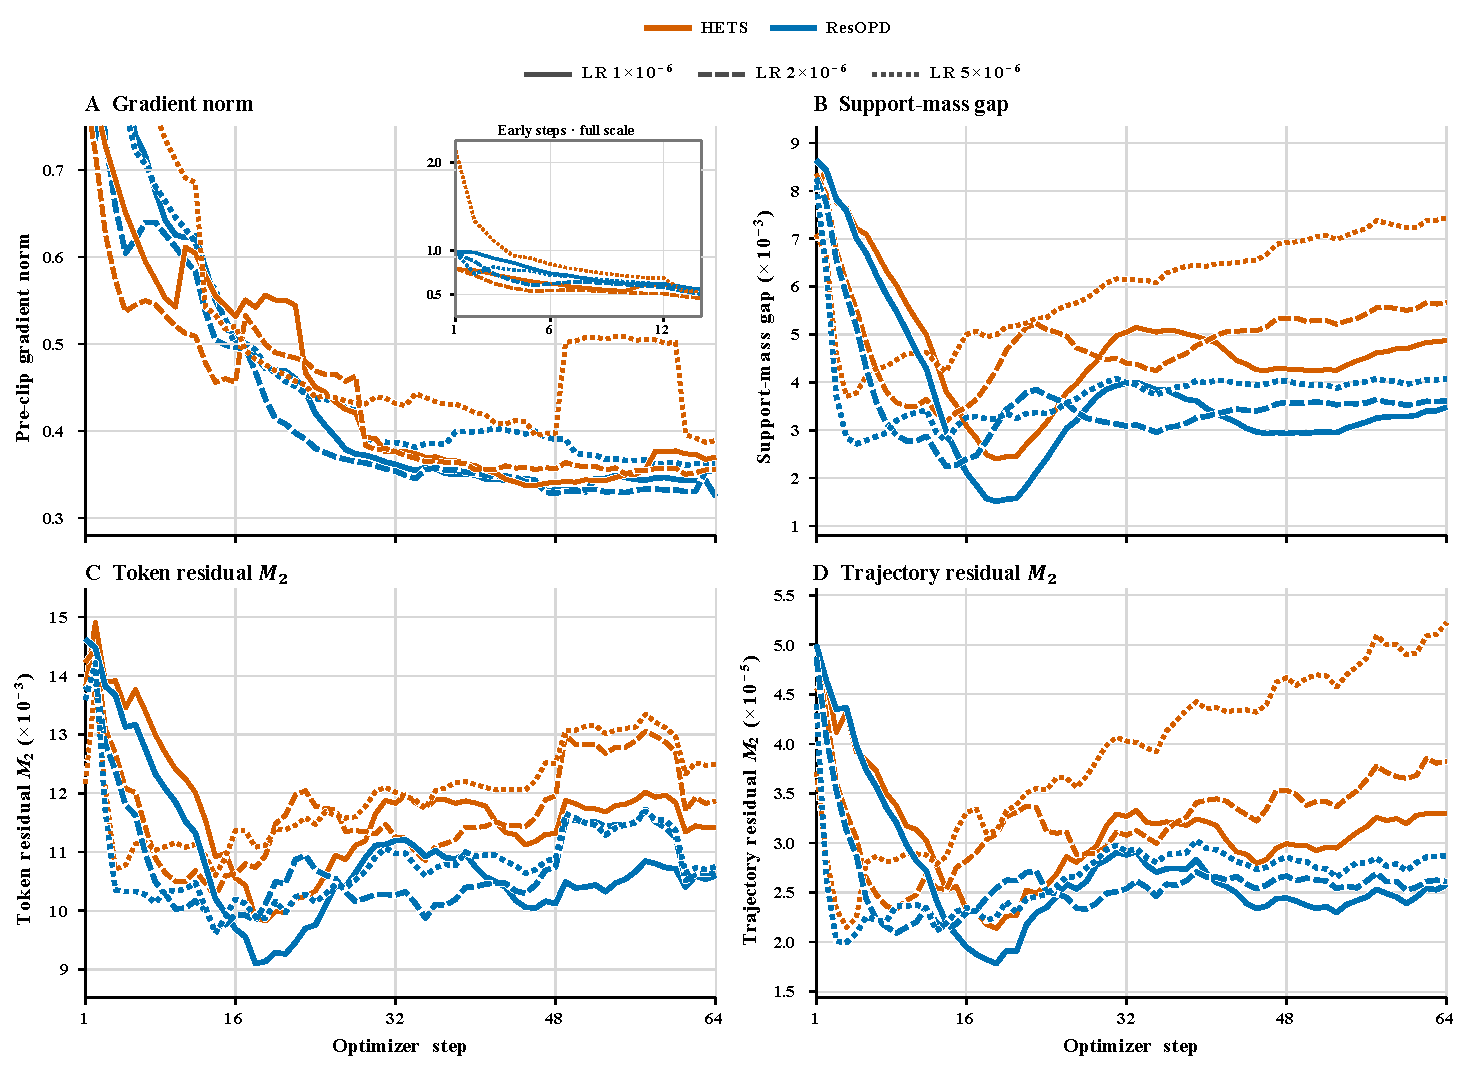
\includegraphics[width=0.9\columnwidth]{figs/lr_training_dynamics_cfr_v3.pdf}
  \caption{\textbf{训练动态与学习率敏感性}：HETS (\textit{橙色}) 与 ResOPD (\textit{蓝色}) 在 DeepMath 上的对比，涵盖三个学习率（$1\times10^{-6}$ 实线，$2\times10^{-6}$ 虚线，$5\times10^{-6}$ 点划线）。
\textbf{(A)} 截断前的全局梯度范数（插图显示早期步骤中完整未截断峰值的全尺度情况）。
\textbf{(B)} 传输教师 Top-4 token 的支持质量差 ($Q - P$ )。
\textbf{(C, D)} token 级别与轨迹级别的二阶残差矩 ($M_2$ )。
当学习率提升至 $5\times10^{-6}$ 时，HETS 表现出显著的梯度范数波动以及逐渐增大的质量/残差差异，而 ResOPD 则保持稳定的动态，并在整个最优化过程中始终贴近其低学习率轨迹。}
  \label{fig:lr-sensitivity}
\end{figure}

\end{document}
